%%
%% This is file `mcmthesis-demo.tex',
%% generated with the docstrip utility.
%%
%% The original source files were:
%%
%% mcmthesis.dtx  (with options: `demo')
%%
%% -----------------------------------
%%
%% This is a generated file.
%%
%% Copyright (C)
%%       2010 -- 2015 by Zhaoli Wang
%%       2014 -- 2019 by Liam Huang
%%       2019 -- present by latexstudio.net
%%
%% This work may be distributed and/or modified under the
%% conditions of the LaTeX Project Public License, either version 1.3
%% of this license or (at your option) any later version.
%% The latest version of this license is in
%%   http://www.latex-project.org/lppl.txt
%% and version 1.3 or later is part of all distributions of LaTeX
%% version 2005/12/01 or later.
%%
%% This work has the LPPL maintenance status `maintained'.
%%
%% The Current Maintainer of this work is Liam Huang.
%%
%%
%% This is file `mcmthesis-demo.tex',
%% generated with the docstrip utility.
%%
%% The original source files were:
%%
%% mcmthesis.dtx  (with options: `demo')
%%
%% -----------------------------------
%%
%% This is a generated file.
%%
%% Copyright (C)
%%       2010 -- 2015 by Zhaoli Wang
%%       2014 -- 2019 by Liam Huang
%%       2019 -- present by latexstudio.net
%%
%% This work may be distributed and/or modified under the
%% conditions of the LaTeX Project Public License, either version 1.3
%% of this license or (at your option) any later version.
%% The latest version of this license is in
%%   http://www.latex-project.org/lppl.txt
%% and version 1.3 or later is part of all distributions of LaTeX
%% version 2005/12/01 or later.
%%
%% This work has the LPPL maintenance status `maintained'.
%%
%% The Current Maintainer of this work is Liam Huang.
%%
\documentclass{mcmthesis}
\mcmsetup{CTeX = false,    % 使用 CTeX 套装时,设置为 true
          tcn = {2518438}, problem = \textcolor{red}{B},
          sheet = true, titleinsheet = true, keywordsinsheet = true,
          titlepage = false, abstract = false}
\usepackage{marginnote}        
\usepackage{newtxtext}     % \usepackage{palatino}
\usepackage[backend=bibtex]{biblatex}   % for RStudio Complie
\usepackage{tabularray}
\usepackage{caption} % for table caption
\usepackage{tocloft}
\usepackage{hyperref}
\usepackage{xcolor}
\usepackage{booktabs} % For cleaner table lines
\usepackage{array}    % For column formatting
\usepackage{caption}
\usepackage{booktabs}   % 三线表支持
\usepackage{siunitx}    % 数值对齐和格式化
\usepackage{caption} 
\usepackage{multirow}
\usepackage{booktabs}
\usepackage{graphicx}
\setlength{\cftbeforesecskip}{6pt}
\renewcommand{\contentsname}{\hspace*{\fill}\Large\bfseries Contents \hspace*{\fill}}

\title{Managing Sustainable Tourism}
% \author{\small \href{http://www.latexstudio.net/}
%   {
\includegraphics[width=7cm]{mcmthesis-logo}}}
\date{\today}

\begin{document}

\begin{abstract}

  We have developed a \textbf{sustainable development model} applicable to the city of Juneau and 
other tourist destinations to address the challenges posed by the rapid growth of tourism
on infrastructure, the natural environment, and resident satisfaction.\par  
For Task 1, we have developed a \textbf{multi-objective optimization model} based on the 
\textbf{Non-dominated Sorting Genetic Algorithm III (NSGA-III)}, where the dual optimization 
objectives are the maximization of economic benefits and the minimization of carbon emissions. 
Economic benefits are quantified through the number of tourists, while carbon emissions 
are used as a \textbf{key indicator of sustainability}. The model introduces three key constraints:  
The \textbf{maximum capacity of infrastructure},
The \textbf{upper limit of tourist numbers},
The \textbf{threshold for resident satisfaction}.
Resident satisfaction is derived from a weighted analysis of dissatisfaction data in the 
survey report, with a 
% \textbf{$15\%$ dissatisfaction threshold} 
limit set based on the actual 
dissatisfaction rate of recent years. 
% $16\%$ in 2023). 
Furthermore, this study has established additional 
expenditure plans covering \textbf{Community projects} by these areas:
\textbf{Environmental protection},
\textbf{Infrastructure development}. \par
For task 2, we classifies different types of tourist destinations through \textbf{cluster analysis}, 
focusing on the differential characteristics of \textbf{core indicators} such as tourist numbers, 
infrastructure carrying capacity, and tourism revenue. Based on the classification results, 
the constraints and parameters of the model are \textbf{dynamically adjusted and optimized} to enhance its 
universality and flexibility, ensuring its applicability to various types of destinations affected 
by overtourism.\par

For task 3, we prepared a \textbf{policy recommendation memorandum} building on the empirical findings to 
provide scientific decision-making support for the sustainable development of tourism in Juneau 
City. The memorandum highlights \textbf{key conclusions} derived from the model's empirical analysis and 
proposes \textbf{actionable policy recommendations}.\par

All in all, the tasks are \textbf{interconnected both theoretically and practically}: Task 1 establishes the \textbf{foundational 
model}, providing methodological support for subsequent research; Task 2 extends and optimizes the 
model, enhancing its \textbf{applicability and scalability}; Task 3 returns to the practical level, offering 
\textbf{empirical evidence} for policy formulation. Innovatively, we have developed a \textbf{scalable optimization 
model} for sustainable tourism development, which not only serves as a decision-making reference for 
Juneau City but also provides a \textbf{replicable analytical framework} and methodological guidance for the 
sustainable development of similar tourist destinations.

\begin{keywords}
  Sustainable Development, NSGA-III, Over-tourism, Multi-objective Optimization
\end{keywords}

\end{abstract}

\maketitle

%% Generate the Table of Contents, if it's needed.
% \renewcommand{\contentsname}{\centering Contents}
\tableofcontents        % 若不想要目录, 注释掉该句
\thispagestyle{empty}

\newpage

\section{Introduction}

\subsection{Background}

As the capital of Alaska, Juneau has a permanent population of approximately $30,000$. In recent years, 
tourism has become a key driver of its economic growth, contributing an annual revenue of approximately 
$\$375$ million. However, the rapid growth of tourism, particularly during peak seasons in Juneau, has led to 
a daily influx of up to $20,000$ visitors.These phenomena pose significant challenges to the local 
social, economic, and environmental fabric. Specifically, issues such as the overburdening of urban 
infrastructure, a decline in residents' quality of life, and environmental degradation have become 
increasingly evident.\par
% Among these challenges, Mendenhall Glacier—one of Juneau's iconic attractions—is facing the dual 
% pressures of global warming and increased carbon emissions resulting from tourism activities, which 
% are accelerating its rate of melting. These not only pose a threat to the long-term appeal of 
% Juneau as a tourist destination, but also raise concerns among local residents about the 
% sustainability of tourism.Besides, the ongoing retreat of the glacier could lead to a decline in 
% tourist numbers, which in turn would undermine the stability of the local economy.\par
In light of these issues, Juneau urgently requires the development and implementation of a 
scientifically-based sustainable tourism strategy that balances economic benefits, tourist 
experience, and environmental conservation. This case study not only highlights the typical 
challenges faced by Juneau as a climate-sensitive tourism destination but also offers valuable 
insights for other regions worldwide grappling with similar issues. The research on the sustainable 
development of Juneau's tourism industry provides both theoretical foundations and practical 
guidance for reconciling the demands of tourism growth with the need for ecological preservation in 
diverse contexts.

\begin{figure}[h] 
  \centering
  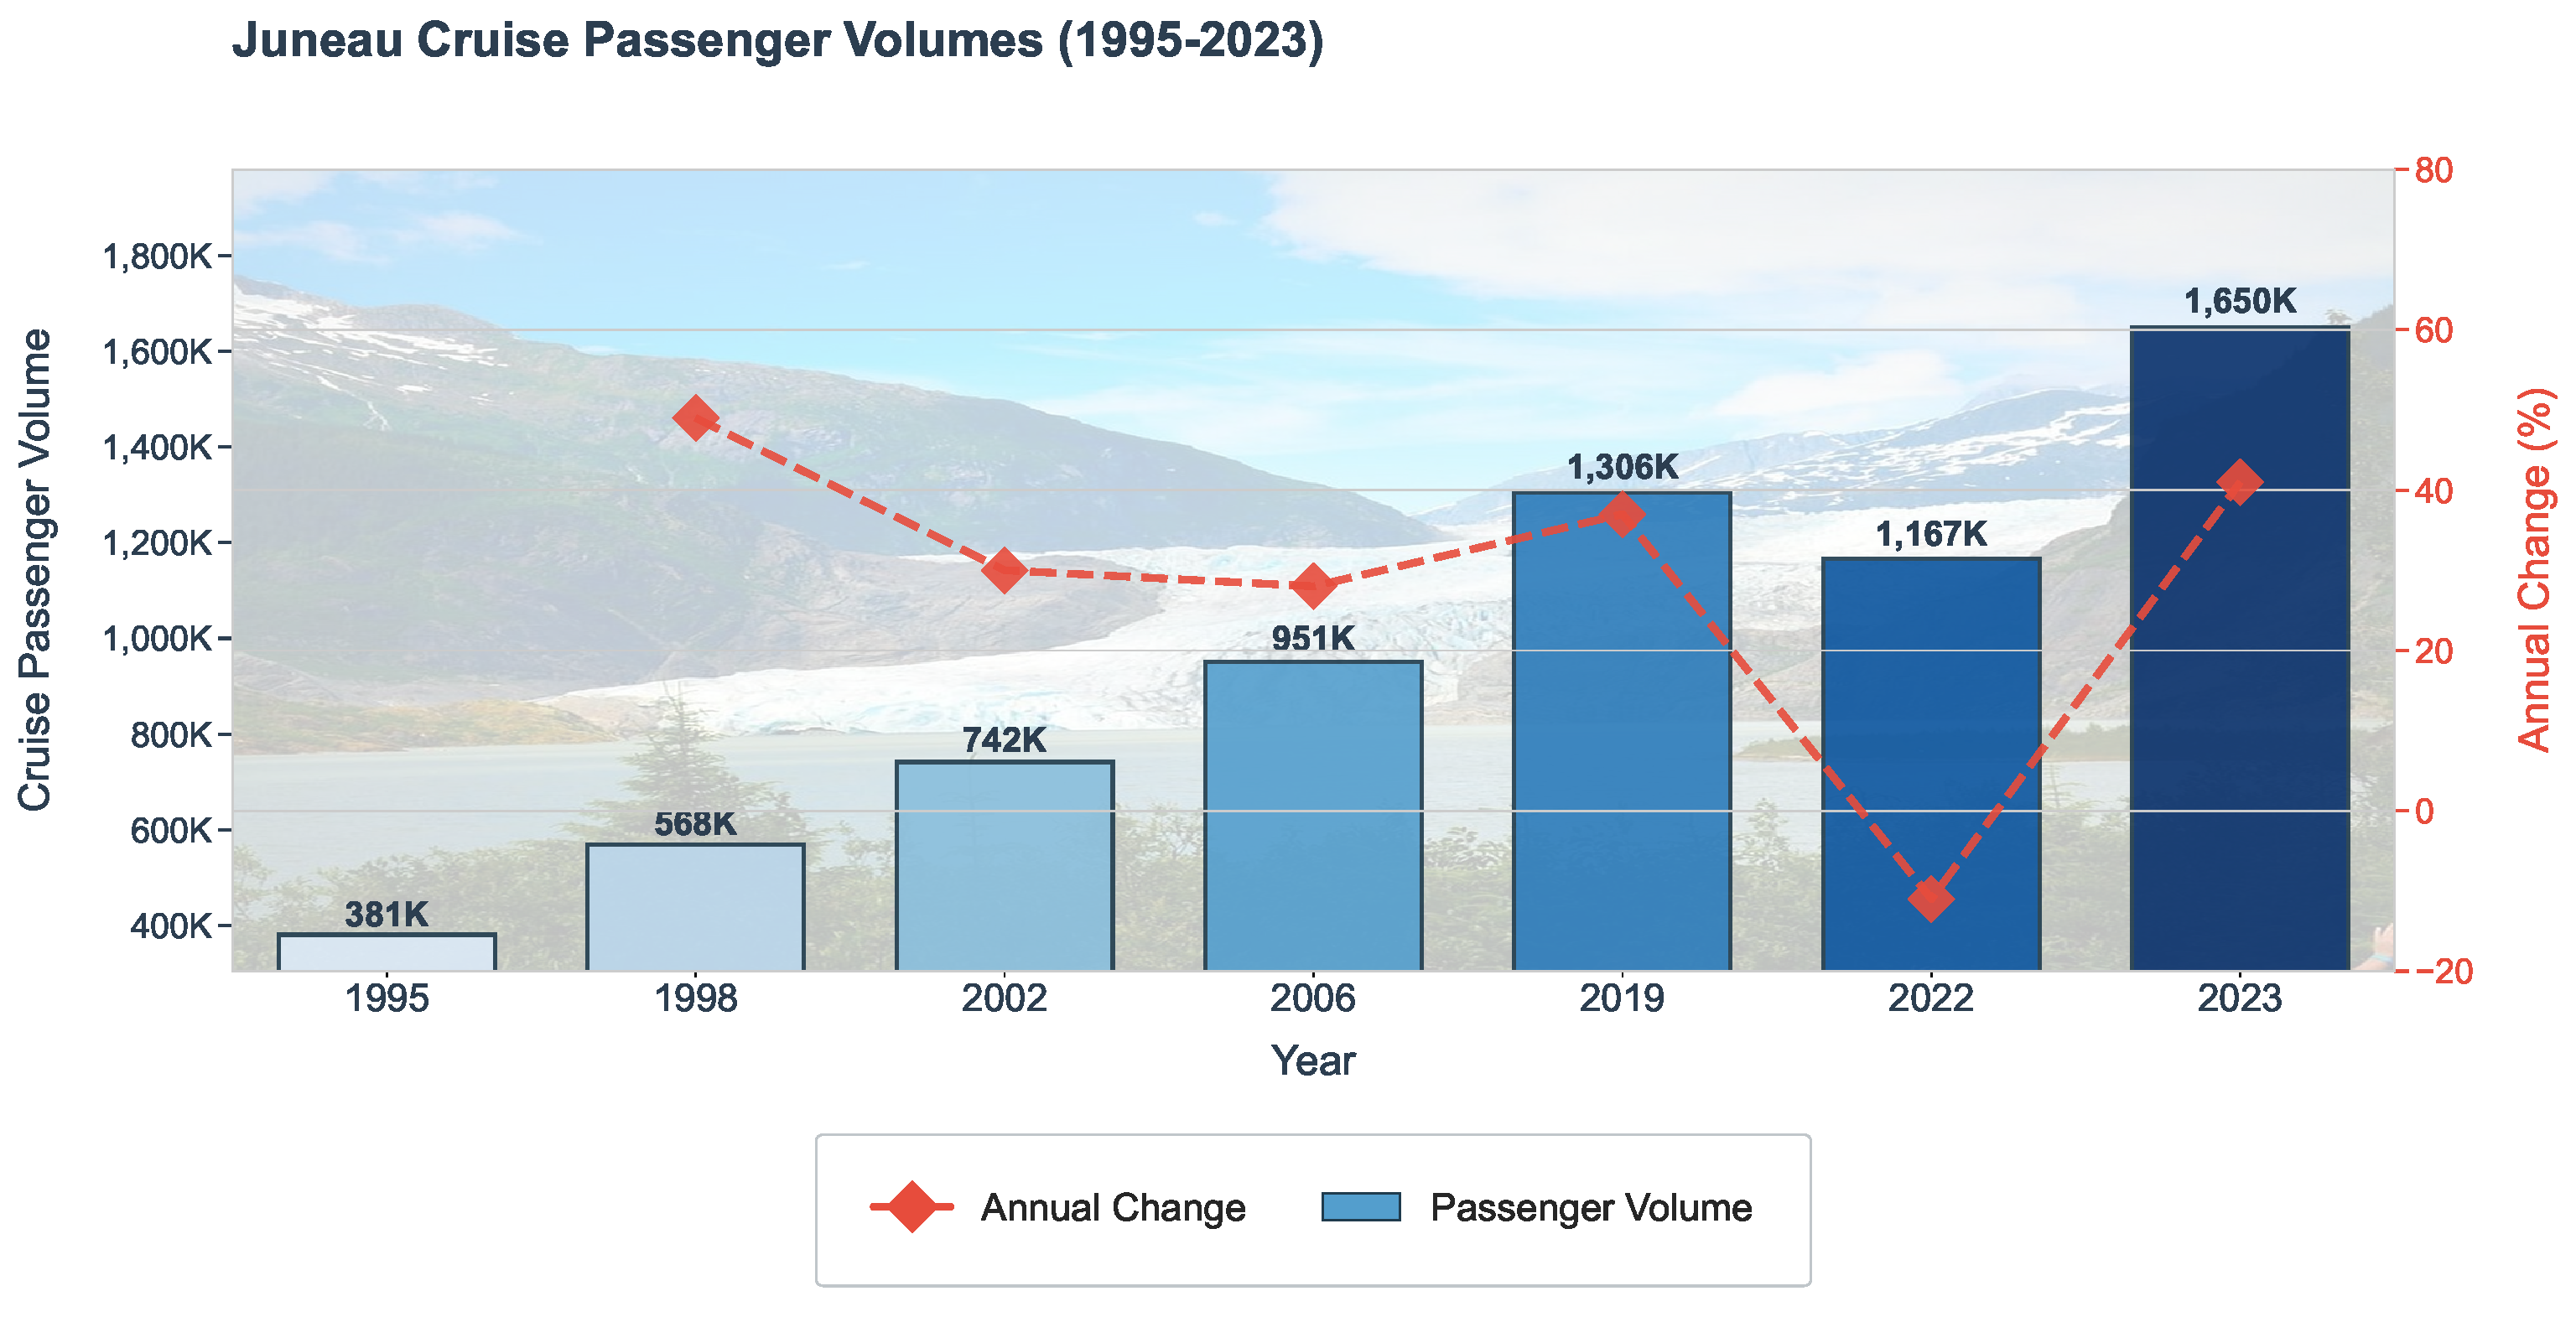
\includegraphics[width=14cm]{totaltour_1.pdf}
  \caption*{Noted: Passenger volumes in 2022 decreased due to COVID-19}\label{fig1}
  \end{figure}

  \subsection{Restatement and Analysis of the Problem}

  We aim to explore key issues in the sustainable development of tourism by constructing a 
  multi-objective optimization model. Our research tasks primarily consist of the following three 
  interrelated aspects:
\begin{itemize}
  \item \textbf{Task 1:  Tourism Sustainability Optimization Framework} This task establishes a comprehensive analytical system combining multivariate regression, input-output analysis, and multi-objective optimization to quantify tourism-environment interactions and optimize investment strategies. Based on literature research and existing survey data, we construct a multiple regression model to examine the relationships between carbon emissions, economic benefits of tourism, glacier melting rates, resident satisfaction, and tourist numbers. Building on this basis, an input-output analysis will be used to assess the investment effectiveness in three areas: environmental protection (carbon reduction), infrastructure development, and community programs. Subsequently, a multi-objective optimization model will be developed using the NSGA-III algorithm. This model will integrate the objective functions and constraints, aiming to determine the optimal tourist carrying capacity and investment allocation plan, followed by a sensitivity analysis of key parameters.
  \begin{figure}[h!] 
    \centering
    \includegraphics[width=12cm]{Work_review02.pdf}
    \caption{Tourism Sustainability Optimization Framework} \label{fig2}
  \end{figure}
  \item \textbf{Task 2: Data-driven adaptability Summary.} This task develops a dynamic clustering methodology to implement differentiated management strategies for diverse tourism destinations. A clustering analysis will be conducted to classify different types of tourist destinations, with a focus on examining the differential characteristics of core indicators such as tourist numbers, infrastructure carrying capacity, and tourism revenue. Based on the classification results, the constraint parameters of the optimization model will be dynamically adjusted to ensure the model's adaptability and flexibility in addressing overtourism impacts at different types of destinations.
  \item \textbf{Task 3: Evidence-based memo writing.} This task translates quantitative findings into actionable governance tools for sustainable tourism management. Based on the empirical research findings, a policy recommendation memorandum will be drafted to provide scientific decision-making support for the sustainable development of Juneau's tourism industry. The memorandum will focus on the key conclusions derived from the model's empirical analysis and offer actionable policy recommendations.
  \end{itemize}
  There is a significant theoretical and practical connection between the tasks outlined above: The foundational model developed in Task 1 provides the methodological support for subsequent research; 

\section{Assumptions and Justification}
To simplify the problem and make it convenient for us to simulate real-life conditions, we
make the following basic assumptions, each of which is properly justified.
\begin{itemize}
  \item \textbf{We conceptualize glacial ablation as an environmental baseline parameter.} 
  Glacial ablation constitutes the principal constraint on regional tourism development as a long-term geomorphic process. 
  $2010-2020$ observations demonstrate sustained annual retreat ($5.9 km^3$) with 
  limited interannual variability. Our passage posits glacial mass balance systems 
  function independently from tourism dynamics, quantifying their tourism impact 
  as an environmental baseline parameter.
\end{itemize}
\section{List of Notation}

\begin{table}[h!]
  \centering
  \begin{tblr}{
    colspec = {X[c]X[c]}, % 自动调整列宽
    cells = {c},
    hline{1-2,9} = {-}{},
  }
  \textbf{Symbol} & \textbf{Meaning} \\
  $V_i$      & Visitor Volume      \\
  $TA^\alpha$      & Tax Allocation in area $\alpha$     \\
  $TR_i$   & Tourism Revenue      \\
  $DS_i$      & Resident Dissatisfaction       \\
  $G_i$        & Glacier Melt Volume      \\
  $C_i$        & Carbon Emissions      \\
  $S_i$  & Infrastructure Stress      
  \end{tblr}
  \caption{List of Notation} 
\end{table}

\section{Data Pre-processing}
\subsection{Data Collection}
Since there is no data provided in the question, we consulted relevant survey 
results and research reports. The data we found about Greenhouse Gas Emissions, Number of Tourists and Total Tourism Revenue from 2011 to 2023 are as Table \ref{tab:tourism}:
% \marginnote{Given the substantial disruptions caused by the COVID-19 pandemic to the tourism sector during 2021-2022, our passage will systematically exclude anomalous observations from this period to ensure analytical validity.}
\begin{itemize}
  \item \textbf{Comprehensive evaluation indicators of tourism industry}\par
  Given that businesses serving the tourism industry also typically cater to the 
  residents of Southeast Alaska, such as restaurants and support services for air and 
  water transportation, it is not feasible to attribute employment and wage data 
  solely to the tourism sector. In the Economic Indicators Reports published annually 
  by the City of Juneau, all positions within the leisure, hospitality, and transportation 
  sectors are aggregated to assess the overall health of the tourism industry. 
  Consequently, the total income reported for the Leisure \& Hospitality sector is 
  considered representative of the total income generated by the tourism industry.
  % ===== 颜色定义 =====
\definecolor{TableHeader}{RGB}{70,130,180}      % 表头颜色 (蓝钢色)
\definecolor{ZebraEven}{RGB}{248,248,248}       % 斑马纹背景 (浅灰)
\definecolor{ColEmission}{RGB}{225,245,255}     % 温室气体列颜色 (极浅蓝)
\definecolor{ColTourists}{RGB}{245,255,230}     % 游客数列颜色 (薄荷绿)
\definecolor{ColRevenue}{RGB}{255,245,210}      % 收入列颜色 (浅鹅黄)
\definecolor{TableLine}{RGB}{220,220,220}       % 表格线颜色
\definecolor{NoteColor}{RGB}{90,90,90}          % 注释文字颜色

\begin{table}[htbp]
  \centering
  \caption{Environmental Impact and Tourism Development (2011-2023)}
  \label{tab:tourism}
  \begin{tblr}{
    width = 0.85\linewidth,
    colspec = {lrrr},
    row{1} = {bg=TableHeader, fg=white, font=\bfseries},  % 表头样式
    row{even} = {bg=ZebraEven},                            % 斑马纹效果
    column{2} = {bg=ColEmission},                          % 第2列背景
    column{3} = {bg=ColTourists},                          % 第3列背景
    column{4} = {bg=ColRevenue},                           % 第4列背景
    hlines = {TableLine},                                  % 水平线样式
    vlines = {},                                           % 无垂直线
    cells = {font=\small},                                 % 统一字号
    cell{2-10}{2-4} = {mode=math},                         % 数学模式
  }
  % ===== 表头 =====
  \SetCell{bg=TableHeader}Year 
    & \SetCell{bg=TableHeader}Greenhouse Gas Emissions 
    & \SetCell{bg=TableHeader}Number of Tourists 
    & \SetCell{bg=TableHeader}Total Tourism Revenue \\
  
  % ===== 单位行 =====
  & (ton CO\textsubscript{2}e) 
    &  
    & (USD) \\
  
  % ===== 数据行 =====
  2011 & 71,727.76    & 1,556,800    & N/A \\
  2012 & 113,587.49   & 1,586,000    & 27,713,469 \\
  2013 & 95,652.89    & 1,693,800    & 28,374,275 \\
  2014 & 76,765.20    & 1,659,600    & 30,711,658 \\
  2015 & 51,892.62    & 1,780,000    & 75,068,464 \\
  2016 & 56,959.98    & 1,857,500    & 79,294,933 \\
  2017 & 49,644.26    & 1,926,300    & 82,318,620 \\
  2018 & 49,236.73    & 2,026,300    & 92,094,125 \\
  2019 & 104,822.60   & 2,213,000    & 103,225,389 \\
  2022 & N/A          & N/A          & 119,520,965 \\
  2023 & N/A          & N/A          & 134,631,332 
  \end{tblr}
  
  % ===== 注释 =====
  \vspace{0.5em}
  {\small\color{NoteColor}\raggedright 
    Data for 2020-2021 affected by COVID-19 are not included.
  }
\end{table}
  \item \textbf{Questionnaire survey on residents' satisfaction}\par
  % From 2011 to 2019, Juneau experienced significant growth in greenhouse gas emissions, tourist 
  % numbers, and tourism revenue. Greenhouse gas emissions peaked in 2012 at $113,587.49$ 
  % tons of CO_2e, later fluctuating, and reached $104,822.60$ tons in 2019, reflecting 
  % tourism's environmental impact. Tourist numbers steadily increased from $1,556,800$ 
  % in 2011 to $2,213,000$ in 2019, which aligns with rising tourism revenue. Revenue 
  % grew sharply from $\$27,713,469$ in 2012 to $\$103,225,389$ in 2019, emphasizing tourism’s 
  % economic contribution. Overall, the rise in tourist numbers and revenue is closely 
  % tied to fluctuations in greenhouse gas emissions, indicating the dual impact of 
  % tourism on Juneau's economy and environment.\par
  We reviewed the tourism satisfaction survey data from the Juneau City Government 
  and plotted the corresponding charts. The results indicate that residents are 
  concerned about tourism-related issues.\par Most are dissatisfied with crowding and 
  sidewalk congestion, with scores between 1 and 2. Regarding overcapacity and 
  visitor limits, attitudes are neutral, with scores between 2 and 3, showing some 
  support but not universal agreement. Traffic congestion is also a concern, with 
  scores mostly between 2 and 3. Cruise frequency and emissions also raise concern, 
  as residents worry about their environmental impact. In contrast, there is strong 
  support for clean energy, with scores concentrated between 4 and 5. Flight emissions 
  also received attention, reflecting concern about the environmental impact of 
  aviation.\par Overall, residents hope tourism can drive economic growth while prioritizing 
  environmental protection. Detailed survey results are shown in Figure \ref{fig:satisfy}.
  \begin{figure}[h] 
    \centering
    {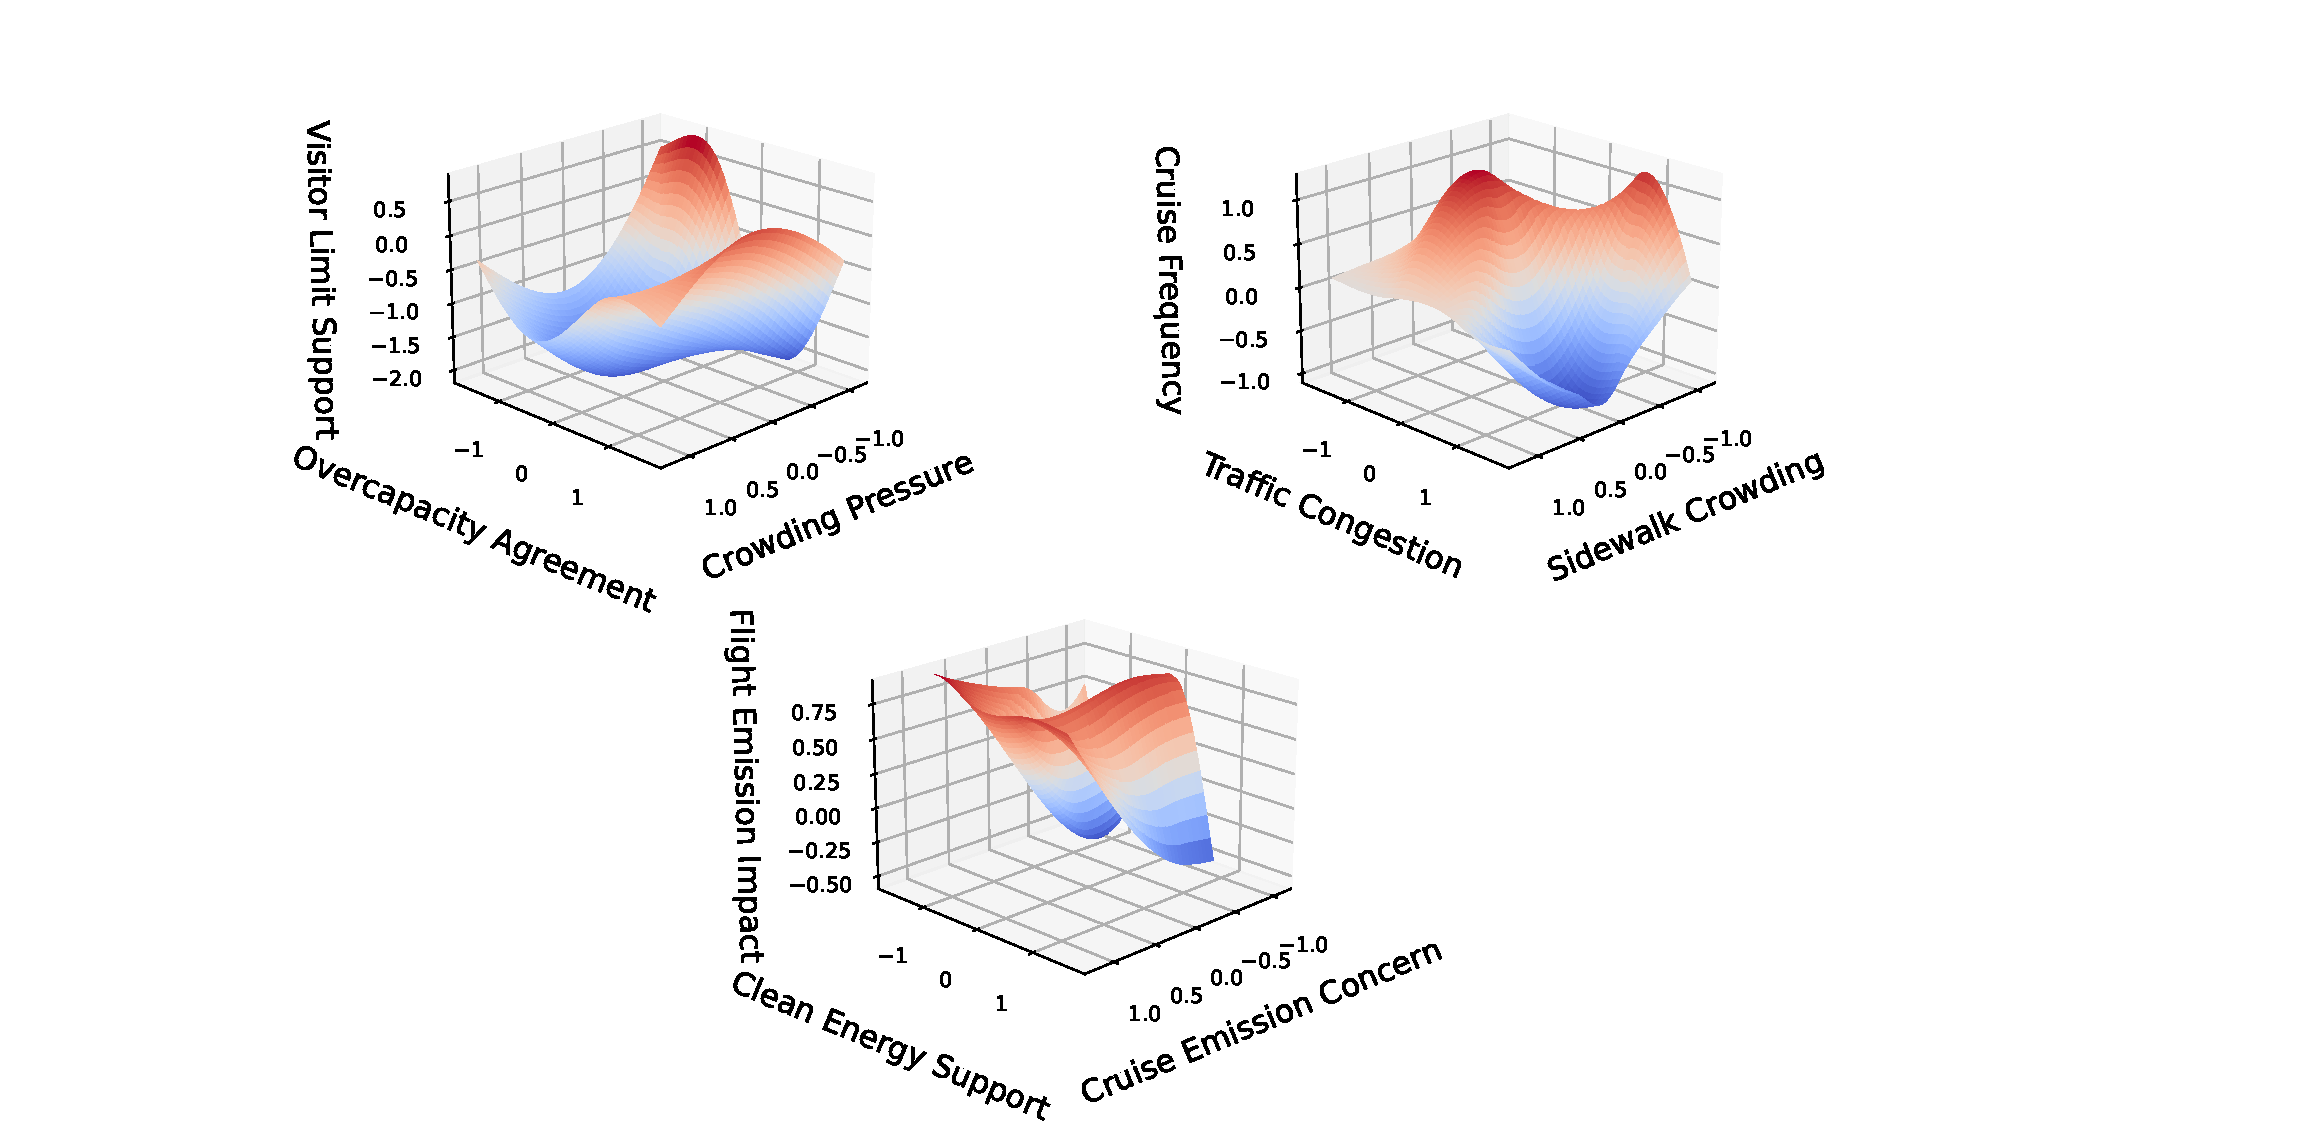
\includegraphics[width=12cm]{Satisfaction Questionnaire.pdf}} % 减小宽度留出边框空间
    \caption{Result of Satisfaction Questionnaire} \label{fig:satisfy}
  \end{figure}
  \item \textbf{Tax income}\par
  We know from the local regulations of Juneau that the local government imposes 9\% Hotel/Motel Tax and 5\% Sales Tax on tourists, with a total tax rate of 14\%. From this, we can conclude that the relationship between local taxes and tourist consumption, that is, local economic income, is:
  $$TA^\alpha = 0.14 \times TR_i$$
  where $TA$ is the total tax income and $TR$ is the total tourism revenue.
  \item \textbf{Calculation of Daily Visitor Distribution}\par
  Based on the annual total of 1,638,902 cruise visitors in Juneau City Port in 2023 and the recorded days exceeding daily visitor thresholds (Table \ref{tab:thresholds}), we assume the daily visitor count
  \begin{table}[h!]
    \centering
    \label{tab:thresholds}
    \rowcolors{2}{gray!10}{white} % 斑马纹:偶数行浅灰填充,奇数行白色
    \begin{tabular}{cc}
      \toprule
      \rowcolor{gray!20} % 单独设置表头背景色
      \textbf{Daily Visitor Threshold (visitors/day)} & \textbf{Days Exceeding Threshold (days)} \\
      \midrule
      5,000  & 40 \\
      6,000  & 40 \\
      7,000  & 39 \\
      8,000  & 37 \\
      9,000  & 30 \\
      10,000 & 25 \\
      11,000 & 22 \\
      12,000 & 15 \\
      13,000 & 13 \\
      14,000 & 9  \\
      15,000 & 6  \\
      16,000 & 4  \\
      17,000 & 3  \\
      18,000 & 2  \\
      19,000 & 1  \\
      \bottomrule
    \end{tabular}
    \caption{Daily Visitor Thresholds and Exceedance Days in 2023}
  \end{table}

  $V^{daily}$ follows a normal distribution $\mathcal{N}(\mu, \sigma^2)$. The probability distribution fitting proceeds as follows:
  $$\mu = \frac{1{,}638{,}902}{365} \approx 4{,}490.1 \, \text{visitors/day}$$
  The daily average visitor count is derived from the annual total.\\
  For each visitor threshold $v^{daily}_i$, its cumulative probability is computed as:
  $$P(V^{daily} \leq v^{daily}_i) = \frac{365 - D_i}{365}$$
  where $D_i$ denotes the number of days exceeding $v^{daily}_i$. The corresponding standard normal quantile is obtained using the inverse cumulative distribution function:
  $$Z_i = \Phi^{-1} \left( P(V^{daily} \leq v^{daily}_i) \right)$$
  A regression relationship between the standardized variable and visitor count is established:
  $$v^{daily}_i - \mu = \sigma Z_i + \epsilon$$
  An intercept-free regression model is employed for fitting, yielding an estimated standard deviation $\sigma = 4589.3$ in Figure \ref{fig:dailyvisitor}.\par
  In summary, the daily tourist volume in Juneau City approximately follows a normal distribution 
  \begin{equation}
    \label{eq:dailyvisitor}
    \mathcal{N}(\mu, (4589.3)^2)
  \end{equation}
  
  
\end{itemize}
% \item 




% \usepackage{color}
% \usepackage{tabularray}
  
\section{Task1: Tourism Sustainability Optimization Framework}
\subsection{Precondition description}
\subsubsection{Relationship between Carbon Emissions and Tourist Numbers}
We selected greenhouse gas emission data from 2011 to 2019 as the dependent variable to examine the dynamic impacts of tourist numbers and temporal factors on emissions. The independent variables were chosen based on the following rationale:
\begin{itemize}
  \item \textbf{Quadratic term of tourist numbers:} Reflects the nonlinear relationship between tourism activities and emissions, capturing changes in marginal effects.
  \item \textbf{Year deviation term ($Year-2011$):} Quantifies cumulative effects of environmental policy implementation while eliminating baseline year selection bias.
  \item \textbf{Data standardization:} Tourist numbers were converted to millions ($V_i^M$) to enhance model stability.
\end{itemize}
Based on this analysis, we established a quadratic regression model with temporal trend:
\begin{equation}
  C_i = \beta_0 + \beta_1 (\text{Year-2011}) + \beta_2 V_i^M + \beta_3 \left( V_i^M \right)^2 + \epsilon 
\end{equation}
\textbf{Through solving the equation, we derived results as shown in the Figure \ref{fig:carbon}}
\begin{figure}[h!]
  \centering
  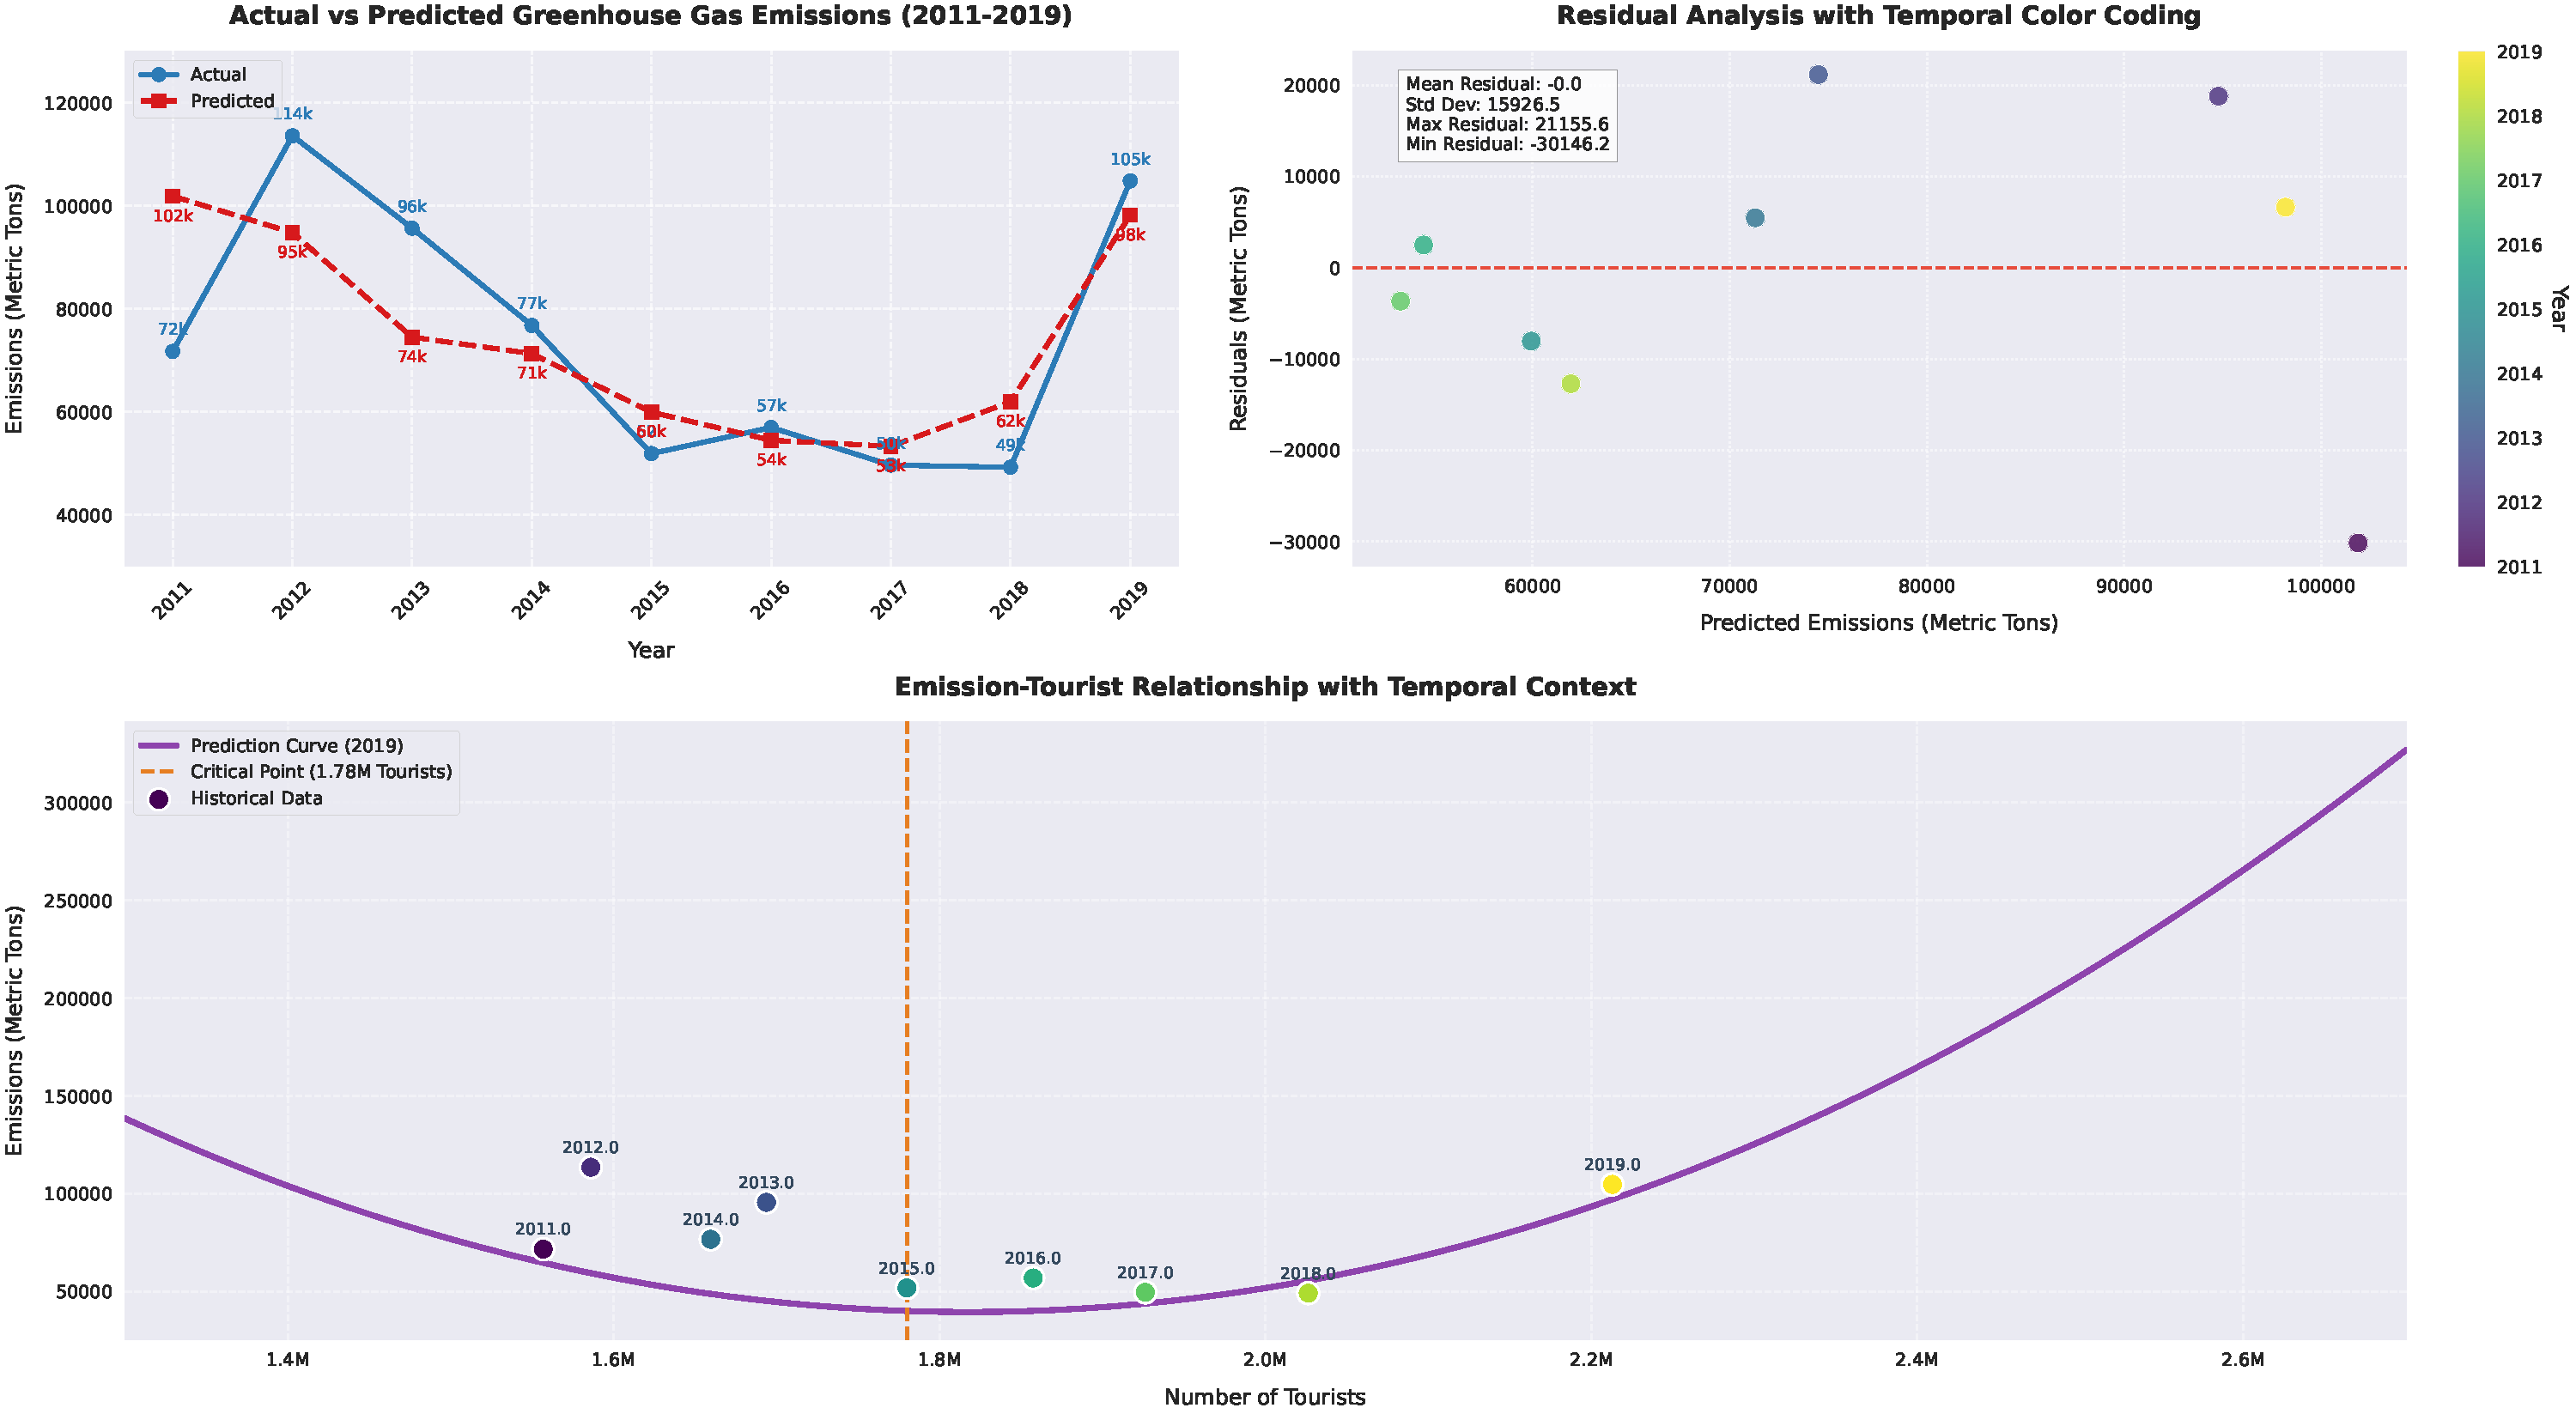
\includegraphics[width=16cm]{tournum-carbon.pdf}
  \caption{Relationship between Carbon Emissions and Tourist Numbers}  % 添加标题
  \label{fig:carbon}                   % 标签放在caption之后
\end{figure}
\begin{itemize}
  \item $\beta_0 = 1,151,001$ represents the baseline intercept for the reference year.
  \item $\beta_1 = −6,723$ quantifies the annual emission reduction effect (unit: metric tons per year).
  \item $\beta_2 = −1,198,962$ and $\beta_3 = 337,702$ jointly capture the nonlinear effects of tourism activities on carbon emissions.
\end{itemize}
\textbf{By deriving the first derivative of this function:}
\begin{equation}
  \frac{\partial C}{\partial V} = \beta_2 + 2\beta_3 V = 0 \quad \Rightarrow \quad V_c = -\frac{\beta_2}{2\beta_3}
\end{equation}
Substituting estimated parameters yields:
\begin{equation}
  V_c = \frac{1,198,962}{2 \times 337,702} \approx 1.78 \text{ million}
\end{equation}
This demonstrates that when Juneau's tourist numbers exceed 1.78 million visitors per year, subsequent growth in tourism will lead to a significant increase in local CO₂ emissions, causing environmental degradation through accelerated glacier melting and other ecological consequences.
\subsubsection{Tourism revenue regression model}
We employed regression analysis to investigate the quantitative relationship between tourist volume and tourism revenue. The linear regression model constructed based on the least squares method is as follows:
\begin{equation}
  TR_i = \beta_0 + \beta_1 V_i + \epsilon
\end{equation}
\textbf{Through regression analysis, the following empirical results were obtained}
\begin{itemize}
  \item \textbf{The regression coefficient $(\beta_1 = 136.581)$}  indicates that for each additional tourist, tourism revenue increases by an average of $\$136.581$. This coefficient quantifies the direct marginal effect of tourist numbers on tourism revenue.
  
  \item \textbf{The intercept term $(\beta_0 = -186,843,122)$} suggests that when tourist numbers equal zero, the predicted tourism revenue would be $\$-186,843,122$, reflecting fixed costs and other unobserved factors affecting the tourism industry in Juneau.
  
  \item \textbf{The coefficient of determination $(R^2 = 0.844)$} demonstrates that the model explains $84.4\%$ of the variance in tourism revenue, indicating a strong goodness-of-fit to the observed data.
  
  \item Statistical significance tests reveal that the regression coefficient exhibits a \textbf{t-statistic of $5.701$} with a corresponding \textbf{p-value of $0.001$}, which is statistically significant at the $\alpha = 0.05$ level. These results confirm a significant linear relationship between tourist numbers and tourism revenue, rejecting the null hypothesis of no association. 
\end{itemize}
\subsubsection{Structural equation model of residents' satisfaction}
Through Structural Equation Modeling (SEM), this study systematically investigates the complex relationships among tourist volume, carbon emissions, glacier status, and satisfaction as Figure \ref{fig:sem}.\\ 
\textbf{The model comprises four latent variables with corresponding observed indicators:}
\begin{itemize}
  \item \textbf{Tourist:} Measured by $Tourist_{Q1}$ (traffic congestion level) and $Tourist_{Q2}$ (cruise frequency), reflecting tourism activity intensity. 
  \item \textbf{Glacier (glacial status):} Evaluated through $Glacier_{Q1}$ (residents' concern about tourism-induced glacial degradation), representing glacial environment protection awareness.
  \item \textbf{Carbon (carbon emissions): } Assessed by $Carbon_{Q1}$ (residents' concern about tourism-related carbon emissions), measuring carbon emission cognition and behavioral patterns.
  \item \textbf{Satisfaction:} Integrated with $Satisfy_{Q1}$ (resident satisfaction), reflecting the interaction between environmental policies and public satisfaction.
\end{itemize}
\textbf{Significance Analysis of Critical Pathways:}\par
The model results demonstrate a statistically significant positive impact of tourist volume on satisfaction (path coefficient: $0.524$, $p < 0.05$). This suggests that increased tourist numbers may enhance overall resident/visitor satisfaction through stimulating local economic vitality or improving infrastructure investment.\par
A significant feedback effect emerges from satisfaction to glacial status (path coefficient: $0.587$,$ **p < 0.01$), indicating that heightened satisfaction may drive stricter glacial protection policies (e.g., tourist capacity restrictions), thereby alleviating glacial pressure.\par
Notably, while the negative impact of carbon emissions on satisfaction lacks statistical significance (path coefficient: $-0.204$, $p > 0.05$), its directional tendency implies potential indirect erosion of public satisfaction through environmental quality deterioration.\par
\textbf{Comprehensive Analysis:}\par
The integrated findings reveal a U-shaped correlation between tourist volume and resident satisfaction. Short-term tourism growth enhances satisfaction through economic benefits, whereas excessive long-term tourism may reduce satisfaction through \textbf{Intensified greenhouse gas emissions} and \textbf{Infrastructure pressure} \par
\begin{figure}[h!] 
  \centering
  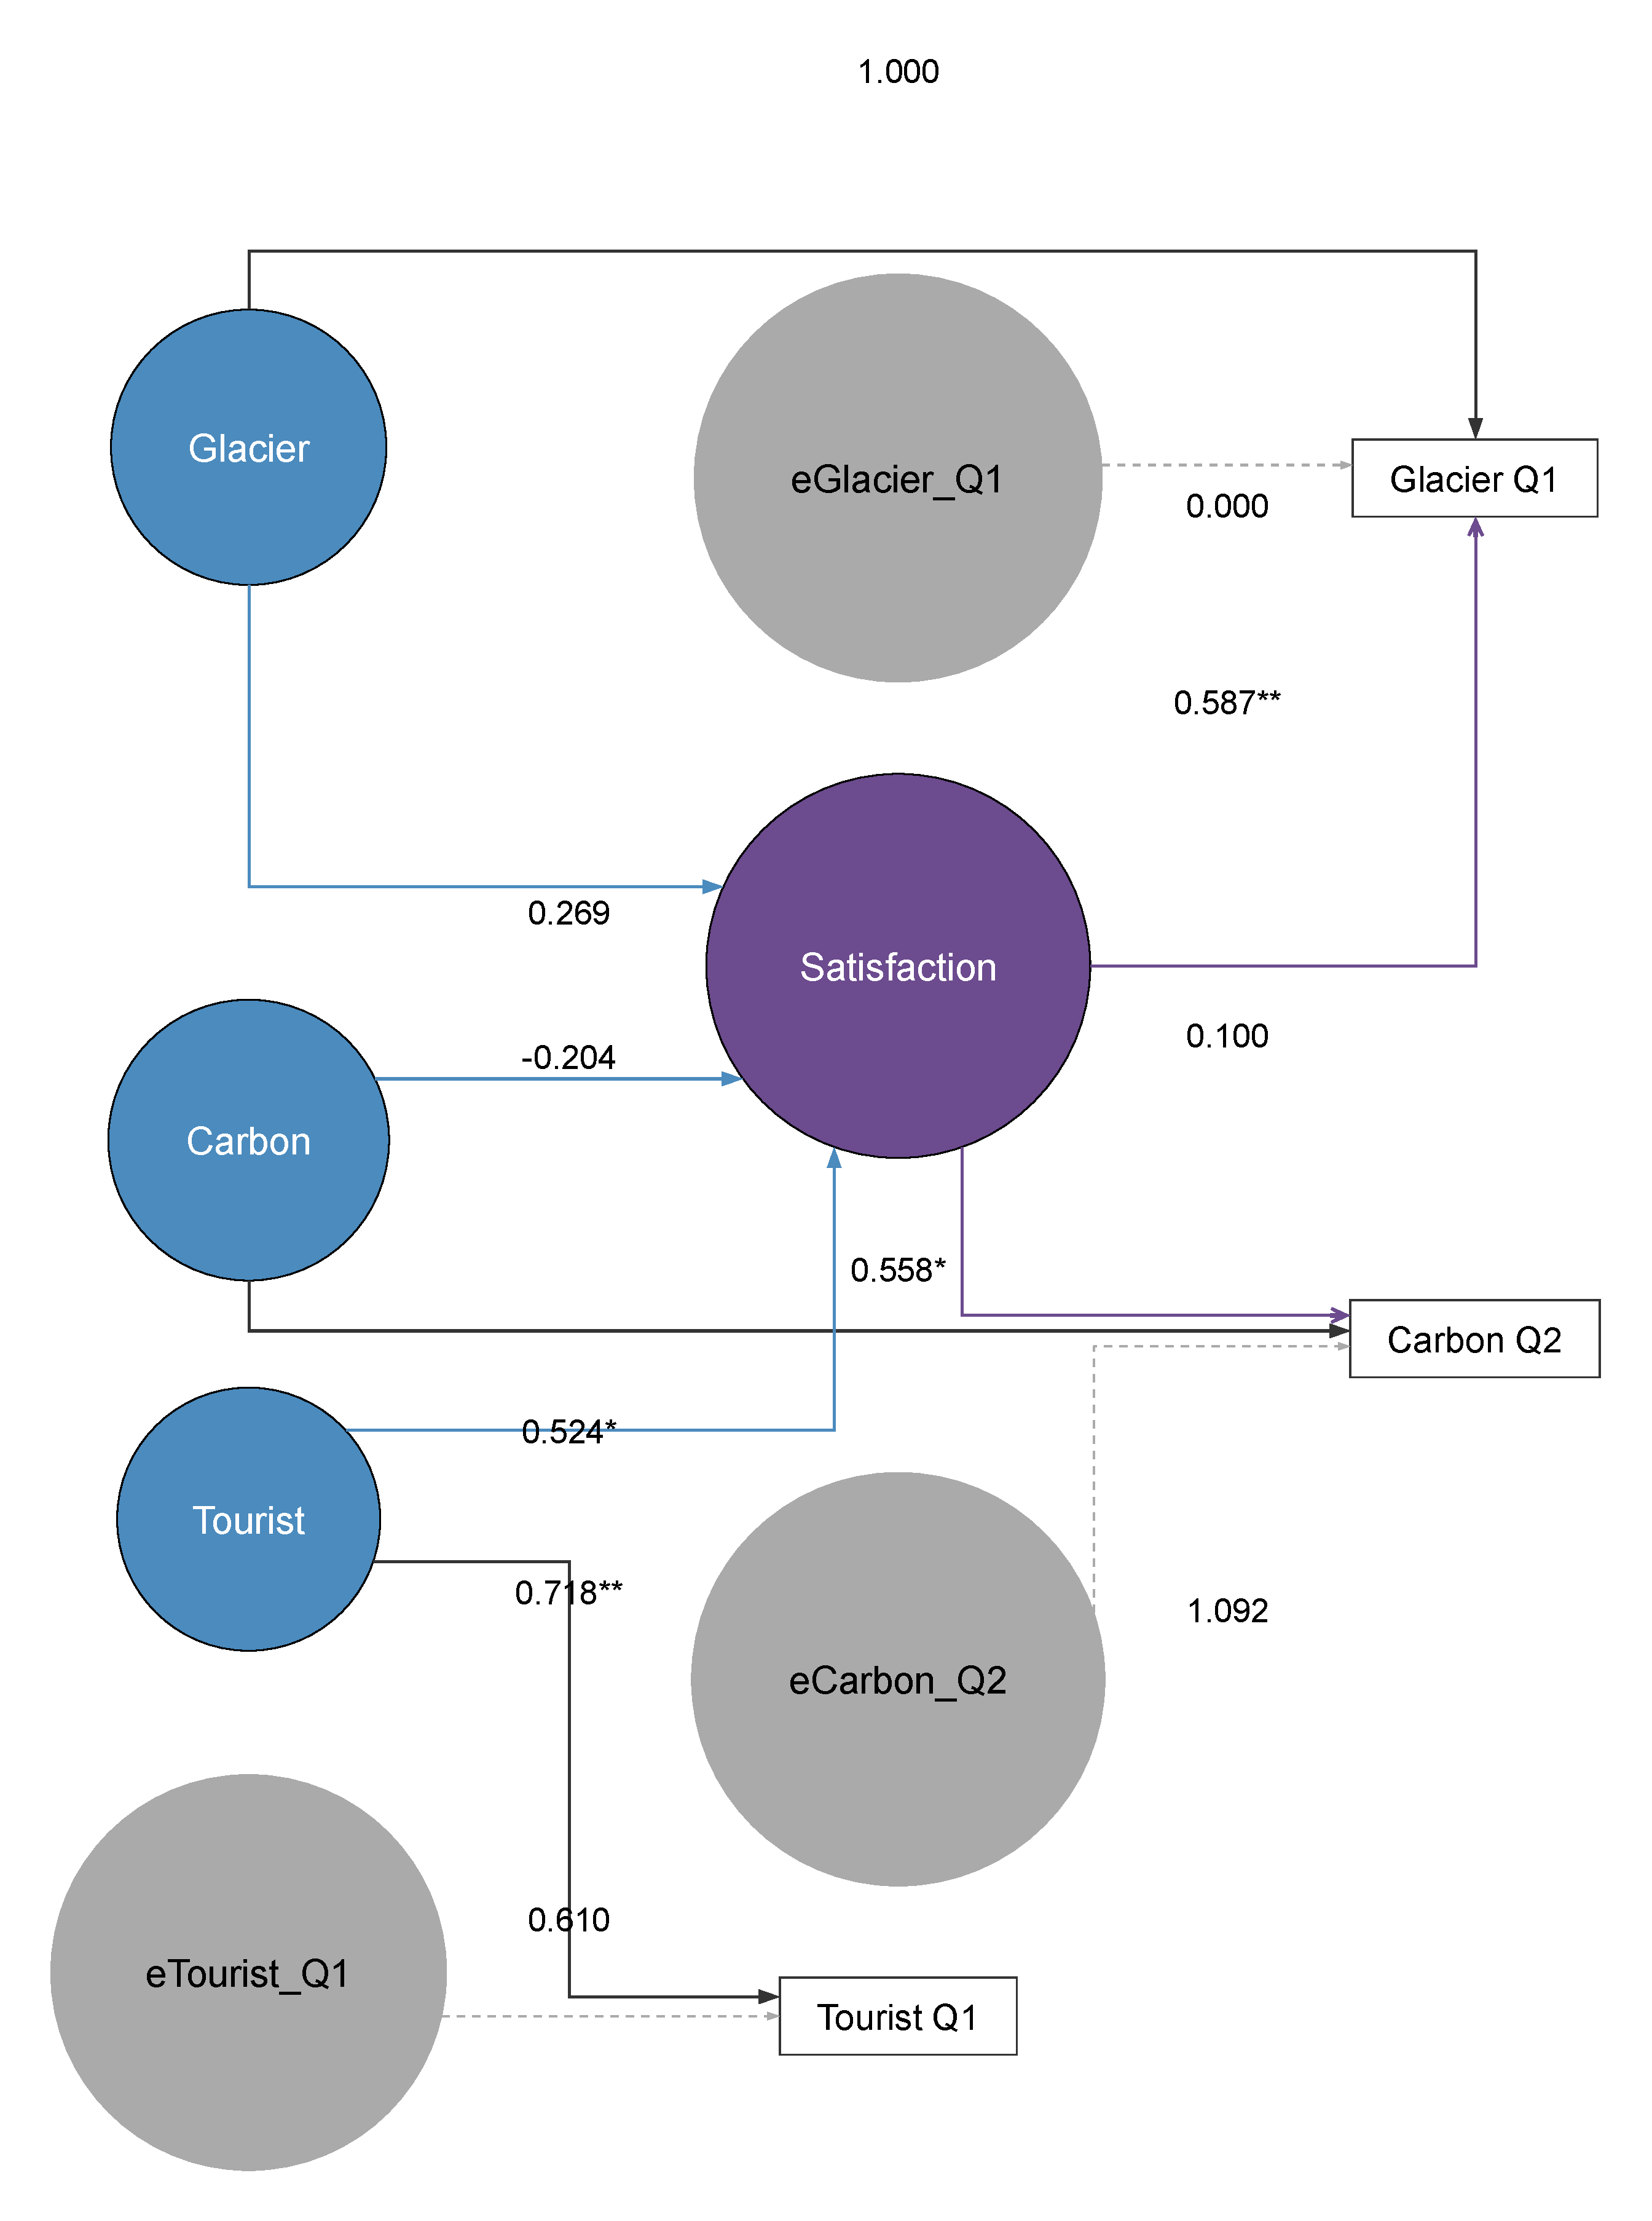
\includegraphics[width=12cm]{sem_diagram_final.pdf}
  \caption{SEM for Resident Satisfaction Surveys} \label{fig:sem}
\end{figure}
All in all,we get the following conclusions:
\begin{equation}
  DS_i = 76.62 - 0.574 V_i^M + 0.0129 \left( V_i^M \right)^2
\end{equation}
\subsubsection{Infrastructure Stress Analysis}
As the majority of tourists visiting Juneau City opt for maritime transportation, the substantial influx of visitors imposes significant strain on the port facilities and adjacent public transportation infrastructure. Based on the 2023 survey report, our analysis indicates that the maximum daily capacity of the port’s traffic system is approximately 14,000 individuals per day. Exceeding this threshold would result in substantial tourist overcrowding. Consequently, we define the transportation infrastructure capacity limit of Juneau City as the condition under which tourist volume remains below this maximum capacity for no more than 97.5\% of days annually. The daily tourist volume is approximated to follow a normal distribution throughout the year as \eqref{eq:dailyvisitor}.\par  
\subsubsection{Input-output of additional expenditure by sector}
We collected relevant information to determine the input-output of additional spending in different areas to determine our additional spending plan.
\begin{itemize}
  \item \textbf{Input-output in the field of carbon emission reduction:} We have examined an environmental justice initiative entitled the Alaska Carbon Reduction Fund, implemented by Renewable Juneau, a non-profit organization based in Juneau. This project allocates funds to replace oil-fired heating systems with high-efficiency, emission-free air-source heat pumps in low-income households. According to disclosed data from the organization, the carbon abatement cost of this initiative amounts to $\$46$ per metric ton of carbon dioxide equivalent $(CO_2e)$ reduced. This metric has been utilized for input-output calculations in the field of carbon emission reduction.
  \item \textbf{Input-output in infrastructure construction:} Based on previous analyses indicating that the substantial tourist influx during peak seasons exerts considerable pressure on Juneau's public transportation system, this study conducts a cost-benefit analysis of infrastructure investments from the perspective of public transportation input-output efficiency.\par
  According to statistical data from the American Public Transportation Association (APTA), the average operational cost of public transit systems in the United States ranges between USD 3-5 per passenger trip. Assuming Juneau's operational costs approximate the national average, with fare revenue covering approximately 50\% of operational expenditures, our calculations demonstrate that each additional passenger served by the transit system would require an incremental investment of USD 200. This derived value results from the differential between total operational costs and fare recovery rates.
\end{itemize} 

\subsection{Model construction and algorithm implementation}
\subsubsection{Multi-objective optimization model construction}
\textbf{Define the 2-dimensional decision variable \( \mathbf{x} = [V_i, TA_{\alpha}] \), where:}
\begin{itemize}
    \item \( V_i \): Annual tourist volume (people/year), range \([0, 4.299 \times 10^6]\)
    \item \( TA_{\alpha} \): Environmental tax allocation ratio (\%), range \([0, 100\%]\)
\end{itemize}

\textbf{Define the objective functions:}
\[
\max \, f_1 = -TR_i = \beta_0 - \beta_1 V_i
\]
\[
\min \, f_2 = C_i = \beta_2 - \beta_3 - \beta_4 V_i + \beta_5 V_i^2 - \frac{TR_i \cdot \beta_6 TA_{\alpha}}{\beta_7}
\]

\textbf{Subject to constraints:}
\[
\begin{cases} 
    g_1 = V_i - \beta_0^1 \leq 0, \\ 
    g_2 = \dfrac{V_i^{\text{cruise}}}{\beta_0^2} + \beta_{1}^2 - S_i \leq 0, \\
    g_3 = \big( \beta_{0}^3 - \beta_{1}^3 V_i + \beta_{2}^3 V_i^2 \big) - \beta_{3}^3 \leq 0,
\end{cases}
\]
\subsubsection{Algorithm selection and parameter setting}
We used the \textbf{NSGA-III algorithm} to solve the optimization problem. The algorithm uses a non-dominated sorting genetic algorithm based on reference points. By systematically generating reference directions, it guides the population to evenly distribute in the target space, avoids the solution set from gathering in local areas, and maintains the diversity and convergence of 
the solution set. 
%Key parameter configurations are shown in Table \ref{tab:params}.
  % For table caption styling
% \begin{table}[!ht]
% \centering
% \caption{Key Parameter Configuration}
% \label{tab:params}

% \begin{tabular}{@{}lll@{}}
% \toprule
% \textbf{Parameter} & \textbf{Value/Method} & \textbf{Theoretical Basis} \\
% \midrule
% Reference Direction Generation Strategy & Das-Dennis Method & Ensure uniform coverage \\
% Number of Reference Directions & 12 & Balance computational efficiency \\
% Population Size & 100 & avoiding premature convergence \\
% Termination Condition & 300 generations & curve indicating steady state \\
% \bottomrule
% \end{tabular}
% \label{tab:params}
% \end{table}
\subsection{Optimization results analysis}
\begin{table}[htbp]
  \centering
  \caption{All Feasible Solutions with Environmental and Economic Indicators}
  \label{tab:solutions}
  \sisetup{
    group-separator = {,},  % 千位分隔符
    table-number-alignment = center,
  }
  \begin{tabular}{
    l  % 新增序号列(左对齐)
    S[table-format=7.0]  % 游客量
    S[table-format=2.2]  % 税收占比
    S[table-format=3.2]  % 经济收益
    S[table-format=6.2]  % 碳排放
  }
  \toprule
  {\textbf{No.}} &  % 新增序号列标题
  {\textbf{Visitor Volume}} & 
  {\textbf{$TA^{environment}$ (\%)}} & 
  {\textbf{Total Revenue (million)}} & 
  {\textbf{Carbon Emissions}} \\
  \midrule
  1  & 2256779 & 50.78 & 121.39 &  52261.30 \\  % 添加序号
  2  & 2530518 & 61.40 & 158.78 & 155696.77 \\
  3  & 2612080 & 56.06 & 169.92 & 200233.36 \\
  4  & 2392205 & 70.76 & 139.89 &  91139.11 \\
  5  & 2556476 & 59.44 & 162.32 & 169469.73 \\
  6  & 2359848 & 71.67 & 135.47 &  78586.32 \\
  7  & 2640759 & 54.34 & 173.83 & 216959.49 \\
  8  & 2449582 & 66.88 & 147.72 & 116217.75 \\
  9  & 2328394 & 76.06 & 131.17 &  65681.00 \\
  10 & 2477035 & 64.55 & 151.47 & 129288.21 \\
  11 & 2503671 & 63.05 & 155.11 & 142148.55 \\  % 原数据中此行游客量应为2503671(原文误为2593671)
  12 & 2584167 & 57.35 & 166.10 & 184714.19 \\
  13 & 2421627 & 68.89 & 143.91 & 103644.60 \\
  \bottomrule
  \end{tabular}
\end{table}
\begin{figure}
  \centering
  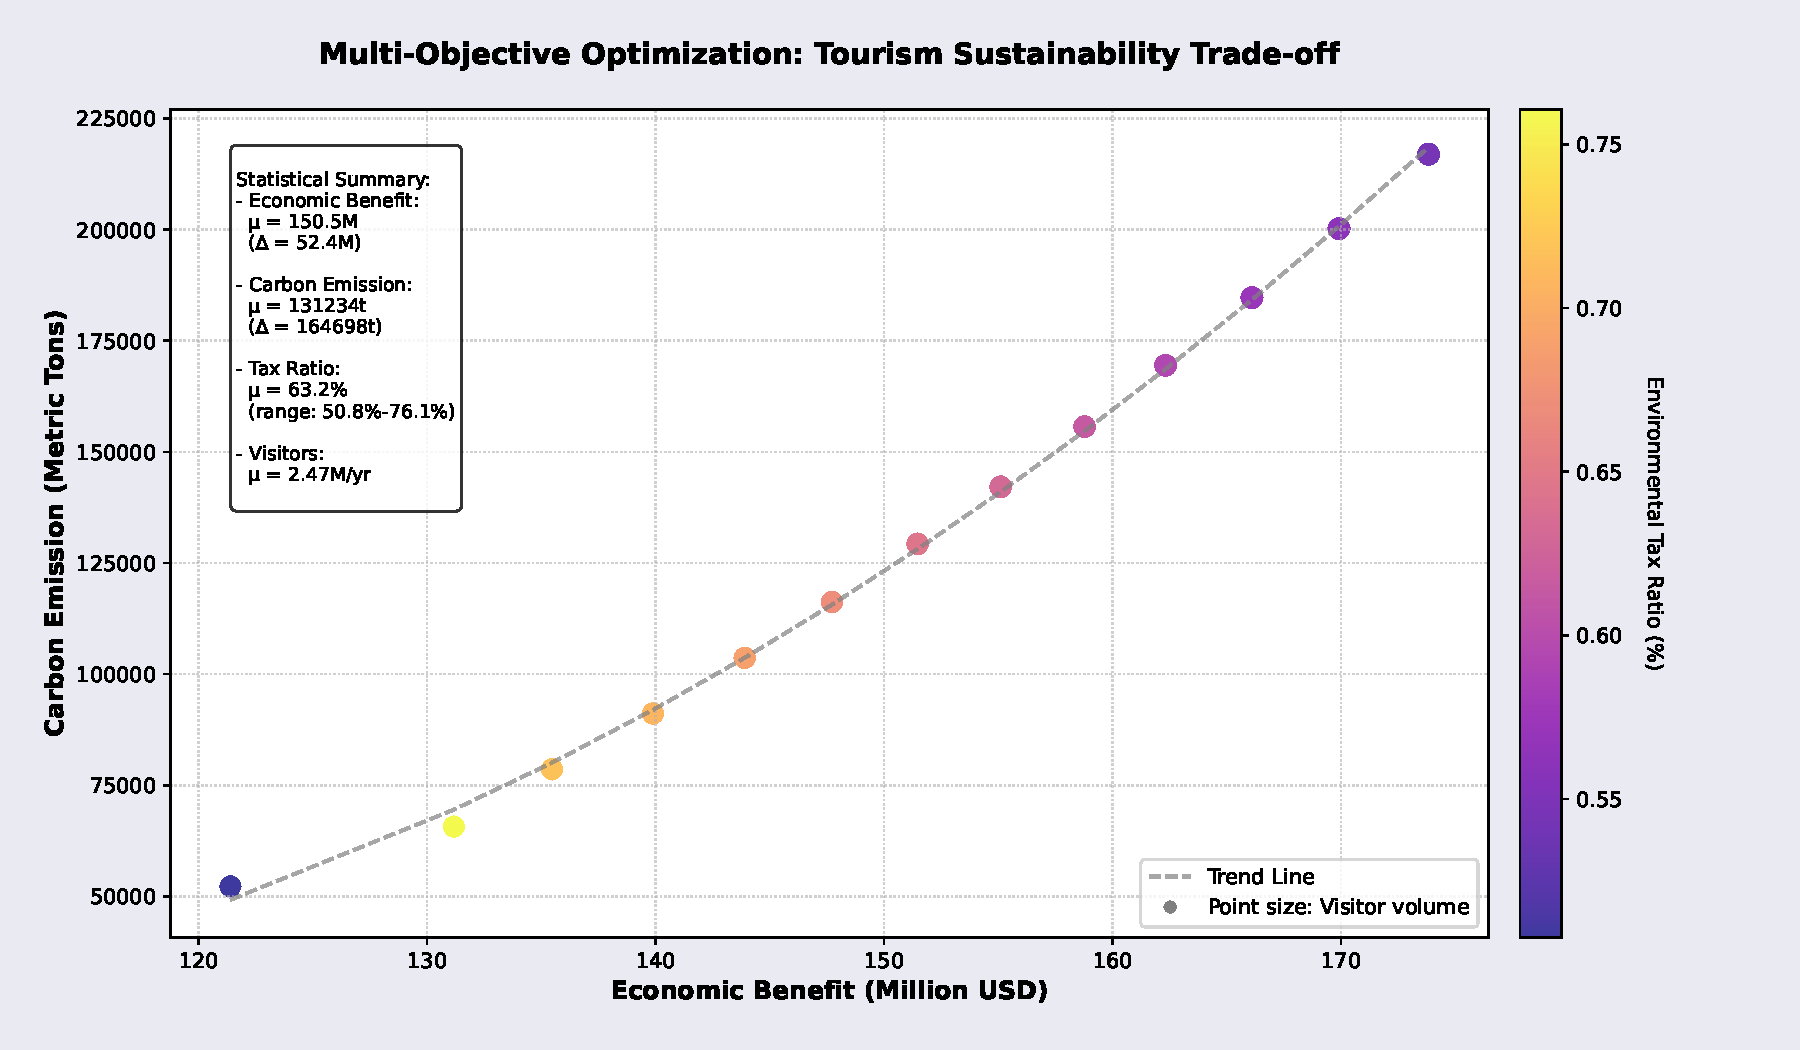
\includegraphics[width=16cm]{NSGA_3_final.pdf}
  \caption{NSGA-III Algorithm Flowchart} \label{fig:nsga}
\end{figure}
Through a comprehensive analysis of 13 sets of feasible solutions (Table \ref{tab:solutions}), significant trade-offs emerge among the indicators of tourist volume, environmental protection expenditure ratio, economic returns, and greenhouse gas emissions across different schemes. From the perspective of economic return maximization, Scheme 7 (2,640,800 annual visitors) achieves the highest economic returns of 173.83 million dollar, but simultaneously exhibits the largest environmental cost with greenhouse gas emissions reaching 216,959.49 tonnes. Scheme 9 (2,328,400 annual visitors) demonstrates optimal sustainability characteristics, featuring the lowest greenhouse gas emissions (65,681.00 tonnes) and the highest environmental protection expenditure ratio (76.06\%), albeit with notably inferior economic returns of 131.17 million dollar.

Notably, Scheme 4 (2,392,200 annual visitors) achieves superior comprehensive benefits: maintaining relatively high economic returns (139.89 million dollar) and environmental protection expenditure ratio (70.76\%) while reducing greenhouse gas emissions (91,139.11 tonnes) to approximately 30\% below the average level. Calculated by carbon emission intensity per unit economic return, this scheme achieves 651.7 tonnes/million dollar, significantly outperforming Scheme 7's 1,248.1 tonnes/million dollar, indicating higher resource utilization efficiency. Additionally, Scheme 6 (2,359,800 annual visitors) demonstrates effective balance between emission control (78,586.32 tonnes) and economic returns (135.47 million dollar), with its environmental protection expenditure ratio reaching 71.67\%, demonstrating sustainable development potential.

In conclusion, Scheme 7 could serve as a short-term strategy prioritizing economic growth. For sustainable development objectives, Schemes 9 and 6 present higher implementation value. For decision-makers pursuing comprehensive benefit maximization, Scheme 4 achieves Pareto improvement by balancing environmental, economic, and fiscal objectives, making it the preferred option.

Considering that Juneau's glacier tourism constitutes a nature-based destination where greenhouse gas emissions accelerate glacial retreat, we recommend adopting Scheme 6 or 9 as tourism development plans. These schemes prioritize environmental protection while maintaining economic balance, thereby achieving green development and sustainable growth.

\begin{table}[htbp]
\centering
\caption{Parameter Comparison of Alternative Schemes}
\label{tab:params}
\begin{tabular}{@{}lcccc@{}}
\toprule
Scheme & Annual Visitors (M) & $TA^{environment}$ (\%) & Total Revenue (million \$) & Emissions (10kt) \\
\midrule
6 & 2.3598 & 71.67 & 135.47 & 7.86 \\
9 & 2.3284 & 76.06 & 131.17 & 6.57 \\
\bottomrule
\end{tabular}
\end{table}


\subsection{Sensitivity analysis}
\textbf{Short-term Motivation} refers to a brief period of above-average performance by a player
following a motivating event (e.g., a breaking serve) during a match, a phenomenon known
in sports as "hot hands". We developed a probabilistic model that quantifies Short-term
Motivation as an increase in serve success rate.\par
The following two assumptions are necessary:
\begin{itemize}
  \item When a player wins a point, he experiences a short-term "motivational" effect that increases
  the probability of winning the next point.
  \item Lifting effects are cumulative. A string of successes may have a positive psychological
  and emotional effect on a player, so that a player winning more points in a row will result
  in a greater probability of winning the next point on serve.
\end{itemize}
Here $i$ denotes the number of consecutive points scored by a player $A$ or his opponent $B$;
and $m_i$ denotes the increase in the rate of serving points on a player’s next serve after winning
$i$points consecutively due to the short-term motivation gained. Then, the probability of winning
the next serve under short-term motivation $p_s$ versus $q_s$ is calculated by \eqref{eq01}.
\begin{equation}
  \begin{split}
    p_s &= p_f(1+m_i^A);\\
    q_s &= q_f(1+m_i^B),
  \end{split}
  \label{eq01}
\end{equation}
where $p_f$ and $q_f$ are the scoring probabilities before player $A$ and player $B$ are motivated,
respectively.\par
The short-term motivation that a player receives for scoring a game $n$ times in a row is
referred to as $n$-order short-term motivation. Using the dataset given in the title, we statistically
obtained a plot of the total number of short-term motivations occurring in a match versus order,
and the results are shown in Figure \ref{fig3}. \par
\begin{figure}[h]
  \centering
  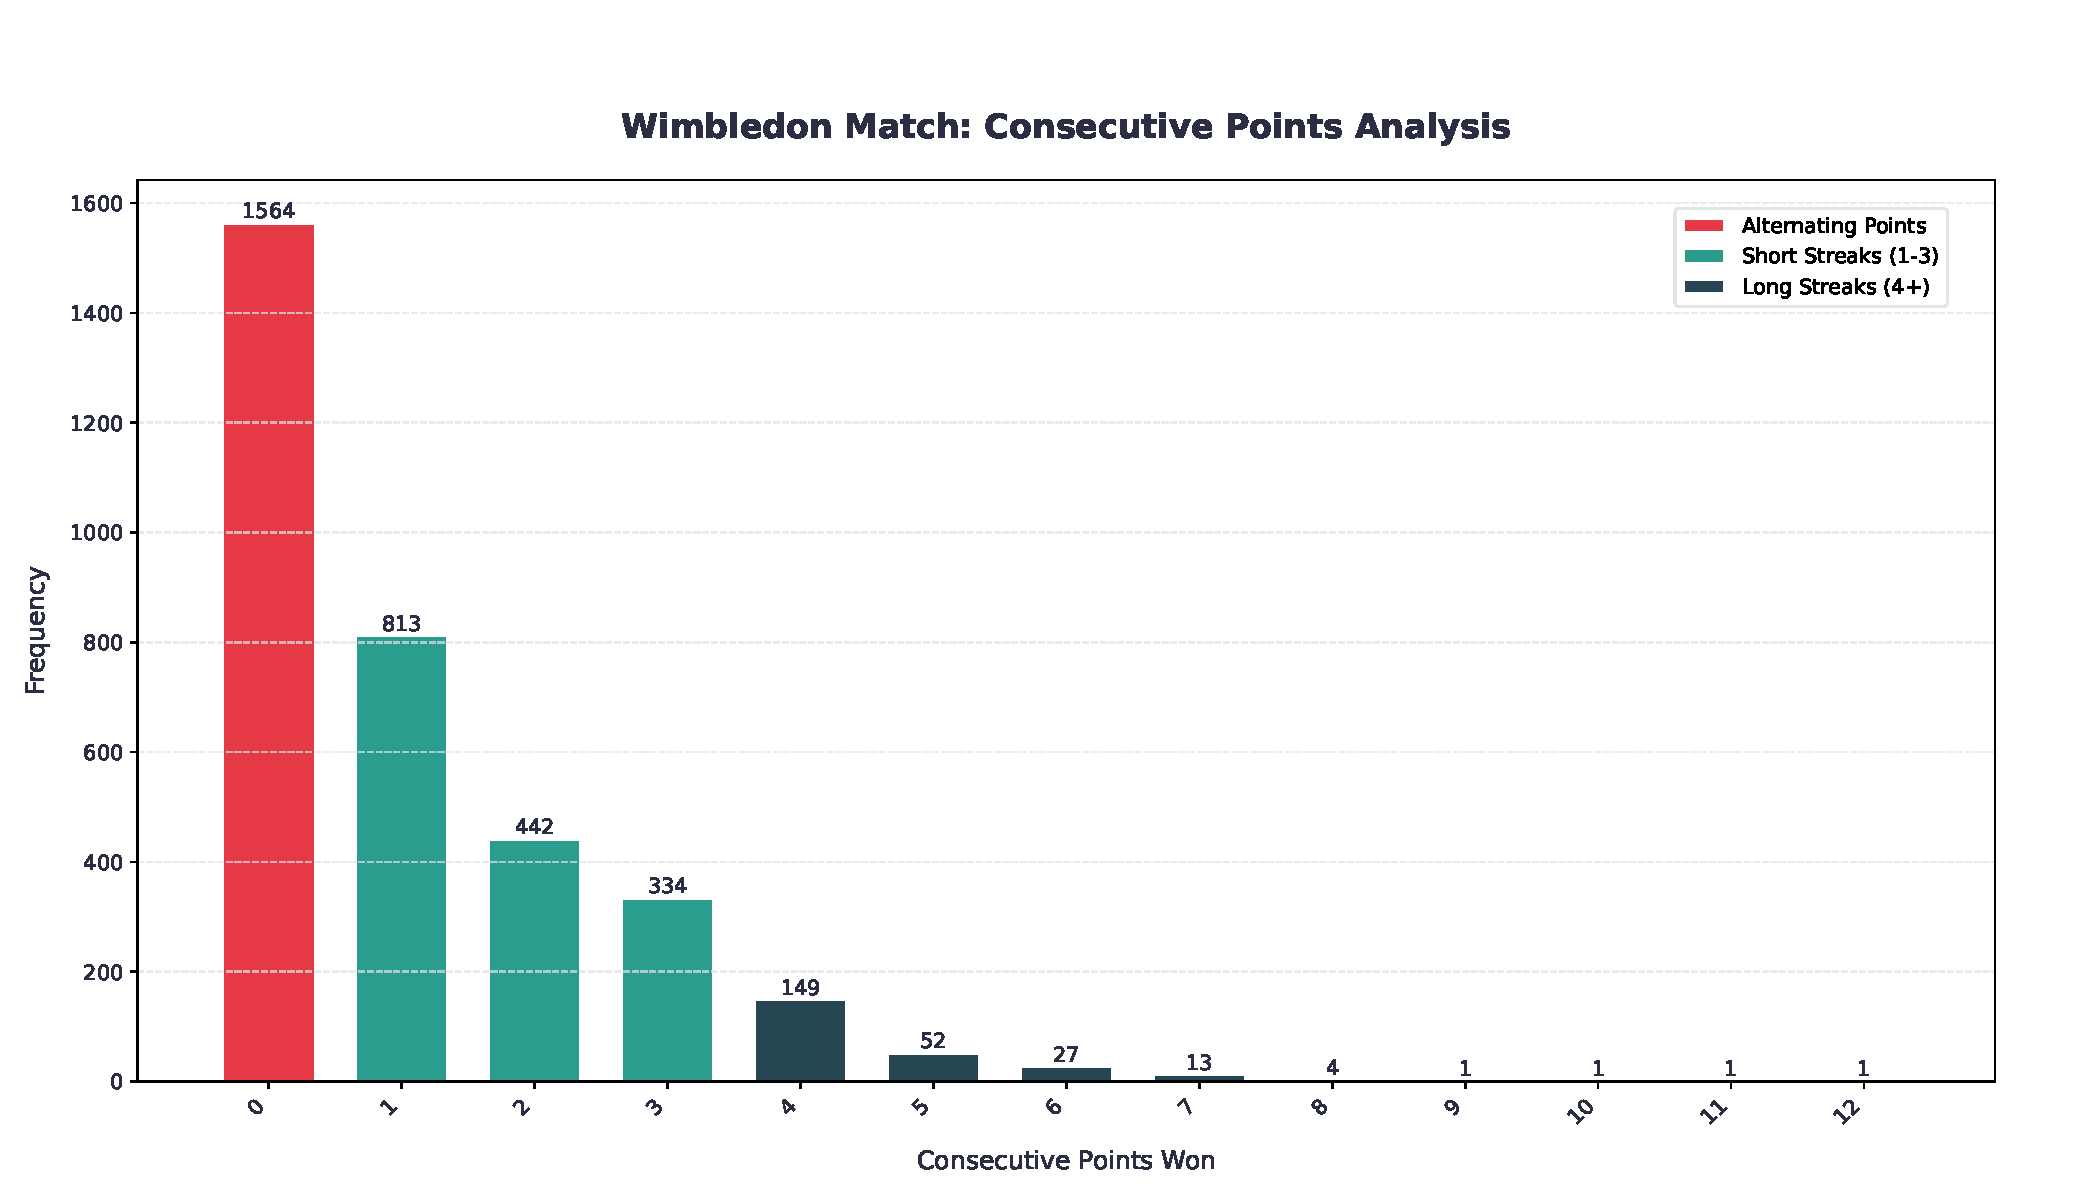
\includegraphics[width=12cm]{continue_winning.pdf}
  \caption{The number of short-term motivations of different orders in a match.} \label{fig4}
  \label{fig3}
\end{figure}
It is clear to see that short-term motivations of order four
and above rarely occur in the dataset used in this study. Therefore, only short-term motivations
of order three and below are considered in this paper.\par
Short-termmotivation focuses on short-termstatus enhancement during matches and ignores
sources of motivation on a longer time scale in the player’s lifetime, so we continue to introduce
a \textbf{confidence-boosting factor}.\par
A new tuning parameter $\lambda$ is introduced, which represents the effect of the confidence
boosting factor on the success rate of the next serve, the probabilities after the effect are
expressed as $p_s$ and $q_s$ – see equation \eqref{eq02}
\begin{equation}
  \begin{split}
    p_c = \frac{T_{AB}}{\lambda} p_t + \left(1 - \frac{T_{AB}}{\lambda}\right) p_0;\\
  q_c = \frac{T_{AB}}{\lambda} q_t + \left(1 - \frac{T_{AB}}{\lambda}\right) q_0,
  \end{split}
  \label{eq02}
\end{equation}
where $T_{AB}$ denotes the cumulative total score of the opposing players since the start of the
match, and $p_t$ and $q_t$ denote the probability of scoring for player $A$ and player $B$, respectively,
since the start of the match up to the present. $p_0$ and $q_0$ denote the historical data on the success
rate of the opposing teams’ serves on the grass court surface prior to the current match (source:
\url{https://www.infosys.com/})\par
Eq. (2) describes the phenomenon that a player’s historical results always have the greatest
impact on player status at the start of a match, and then diminish as the match progresses - the
performance of the current match begins to influence player play more.\par
We then performed a linear interpolation of the obtained probabilities. The interpolation
coefficient is the cumulative total score of the current pair divided by the coefficient $\lambda$ (i.e.$\frac{T_{AB}}{\lambda}$).\par
The short-term motivation is fluctuating as the match progresses, while the confidence boost
takes into account the player’s self-perception established over the course of his career as well
as the current situation in the match, which is the "undertone" of the motivated state, therefore,
we use $pc$ and $qc$ in Eq. \eqref{eq02} instead of $p_f$ and $q_f$ in Eq. \eqref{eq01}, we can get the success rate of the
next serve after considering the short-term motivation and confidence improvement:
\begin{equation*}
  \begin{split}
    p = \left[ \frac{T_{AB}}{\lambda} \cdot p_c + \left( 1 - \frac{T_{AB}}{\lambda} \right) p_t \right] (1 + m_i^A);\\
    q = \left[ \frac{T_{AB}}{\lambda} \cdot q_c + \left( 1 - \frac{T_{AB}}{\lambda} \right) q_t \right] (1 + m_i^B).
  \end{split}
\end{equation*}
The above equation shows the effect of short-term motivation and confidence enhancement
on serve percentage.\par
In tennis matches, players typically have an advantage when serving. According to the
data we have collected, the serving success rate of professional players exceeds $50\%$. Based
on this understanding, \textbf{players gain confidence in serving games.} Due to this "confidence
boost," we have incorporated the player’s performance in serving games into consideration in
our model.
\subsubsection{Monte Carlo Simulation for Winning Probability}
As a sports competition, there is a great deal of uncertainty in tennis, for which Monte Carlo
algorithms can provide probabilistic estimates of the outcome.\par
Based on the serve success rate obtained in the previous section, we use the Monte Carlo
algorithm to simulate each ball, and ultimately obtain the winners and losers of each game, set
and even the whole match. Then in this process, the randomness and diversity of the simulation
are ensured by generating a large number of random number seeds.\par
Here is the pseudo-code for the algorithm we used:\par
\begin{center}
\begin{tabular}{clc}
{\bf Symbols} & {\bf Description} & \quad {\bf Unit} \\[0.25cm]
$h$ & Convection heat transfer coefficient & \quad W/(m$^2 \cdot$ K) 
\\[0.2cm]
$k$ & Thermal conductivity & \quad W/(m $\cdot$ K) \\[0.2cm]
$c_p$ & Specific heat & \quad J/(kg $\cdot$ K) \\[0.2cm]
$\rho$ & Density & \quad kg/m$^2$ \\[0.2cm]
$\delta$ & Thickness & \quad m \\[0.2cm]
$t$ & Temperature & \quad $^\circ$C, K \\[0.2cm]
$\tau$ & Time & \quad s, min, h \\[0.2cm]
$q_m$ & Mass flow & \quad kg/s \\[0.2cm]
$\Phi$ & Heat transfer power & \quad W \\[0.2cm]
$T$ & A period of time & \quad s, min, h \\[0.2cm]
$V$ & Volume & \quad m$^3$, L \\[0.2cm]
$M,\,m$ & Mass & \quad kg \\[0.2cm]
$A$ & Aera & \quad m$^2$ \\[0.2cm]
$a,\,b,\,c$ & The size of a bathtub  & \quad m$^3$
\end{tabular}
\end{center}

\noindent where we define the main parameters while specific value of those parameters will be given later.

\section{Model Overview}

In our basic model, we aim at three goals: keeping the temperature as even as possible, making it close to the initial temperature and decreasing the water consumption.

We start with the simple sub-model where hot water is added constantly.
At first we introduce convection heat transfer control equations in rectangular coordinate system. Then we define the mean temperature of bath water.

Afterwards, we introduce Newton cooling formula to determine heat transfer
capacity. After deriving the value of parameters, we get calculating results via formula deduction and simulating results via CFD.

Secondly, we present the complicated sub-model in which hot water is
added discontinuously. We define an iteration consisting of two process:
heating and standby. As for heating process, we derive control equations and boundary conditions. As for standby process, considering energy conservation law, we deduce the relationship of total heat dissipating capacity and time.

Then we determine the time and amount of added hot water. After deriving the value of parameters, we get calculating results via formula deduction and simulating results via CFD.

At last, we define two criteria to evaluate those two ways of adding hot water. Then we propose optimal strategy for the user in a bathtub.
The whole modeling process can be shown as follows.

\begin{figure}[h] 
\centering
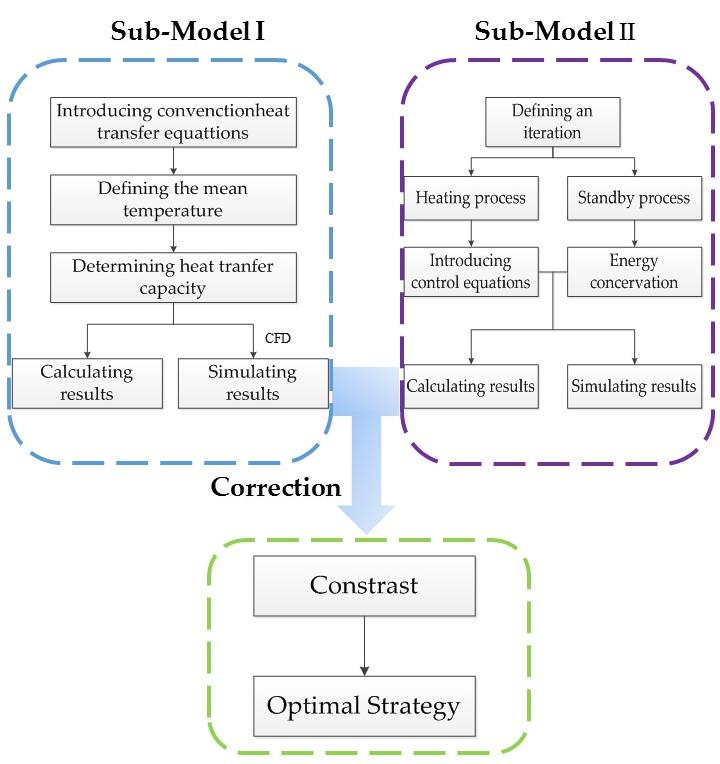
\includegraphics[width=12cm]{fig1.jpg}
\caption{Modeling process} \label{fig1}
\end{figure}

\section{Sub-model I : Adding Water Continuously}

We first establish the sub-model based on the condition that a person add water continuously to reheat the bathing water. Then we use Computational Fluid Dynamics (CFD) to simulate the change of water temperature in the bathtub. At last, we evaluate the model with the criteria which have been defined before.

\subsection{Model Establishment}

Since we try to keep the temperature of the hot water in bathtub to be even, we have to derive the amount of inflow water and the energy dissipated by the hot water into the air.

We derive the basic convection heat transfer control equations based on the former scientists’ achievement. Then, we define the mean temperature of bath water. Afterwards, we determine two types of heat transfer: the boundary heat transfer and the evaporation heat transfer. Combining thermodynamic formulas, we derive calculating results. Via Fluent software, we get simulation results.

\subsubsection{Control Equations and Boundary Conditions}

According to thermodynamics knowledge, we recall on basic convection
heat transfer control equations in rectangular coordinate system. Those
equations show the relationship of the temperature of the bathtub water in space.

We assume the hot water in the bathtub as a cube. Then we put it into a
rectangular coordinate system. The length, width, and height of it is $a,\, b$ and $c$.

\begin{figure}[h] 
\centering
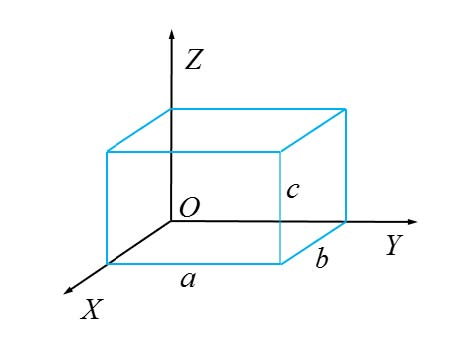
\includegraphics[width=8cm]{fig2.jpg}
\caption{Modeling process} \label{fig2}
\end{figure}

In the basis of this, we introduce the following equations \cite{5}:

\begin{itemize}
\item {\bf Continuity equation:}
\end{itemize}

\begin{equation} \label{eq1}
\frac{\partial u}{\partial x} + \frac{\partial v}{\partial y} +\frac{\partial w}{\partial z} =0
\end{equation}

\noindent where the first component is the change of fluid mass along the $X$-ray. The second component is the change of fluid mass along the $Y$-ray. And the third component is the change of fluid mass along the $Z$-ray. The sum of the change in mass along those three directions is zero.

\begin{itemize}
\item {\bf Moment differential equation (N-S equations):}
\end{itemize}

\begin{equation} \label{eq2}
\left\{
\begin{array}{l} \!\!
\rho \Big(u \dfrac{\partial u}{\partial x} + v \dfrac{\partial u}{\partial y} + w\dfrac{\partial u}{\partial z} \Big) = -\dfrac{\partial p}{\partial x} + \eta \Big(\dfrac{\partial^2 u}{\partial x^2} + \dfrac{\partial^2 u}{\partial y^2} + \dfrac{\partial^2 u}{\partial z^2} \Big) \\[0.3cm]
\rho \Big(u \dfrac{\partial v}{\partial x} + v \dfrac{\partial v}{\partial y} + w\dfrac{\partial v}{\partial z} \Big) = -\dfrac{\partial p}{\partial y} + \eta \Big(\dfrac{\partial^2 v}{\partial x^2} + \dfrac{\partial^2 v}{\partial y^2} + \dfrac{\partial^2 v}{\partial z^2} \Big) \\[0.3cm]
\rho \Big(u \dfrac{\partial w}{\partial x} + v \dfrac{\partial w}{\partial y} + w\dfrac{\partial w}{\partial z} \Big) = -g-\dfrac{\partial p}{\partial z} + \eta \Big(\dfrac{\partial^2 w}{\partial x^2} + \dfrac{\partial^2 w}{\partial y^2} + \dfrac{\partial^2 w}{\partial z^2} \Big)  
\end{array}
\right.
\end{equation}

\begin{itemize}
\item {\bf Energy differential equation:}
\end{itemize}

\begin{equation} \label{eq3}
\rho c_p \Big( u\frac{\partial t}{\partial x} + v\frac{\partial t}{\partial y} + w\frac{\partial t}{\partial z} \Big) = \lambda \Big(\frac{\partial^2 t}{\partial x^2} + \frac{\partial^2 t}{\partial y^2} + \frac{\partial^2 t}{\partial z^2} \Big)
\end{equation}

\noindent where the left three components are convection terms while the right three components are conduction terms.

By Equation \eqref{eq3}, we have ......

......

On the right surface in Fig. \ref{fig2}, the water also transfers heat firstly with bathtub inner surfaces and then the heat comes into air. The boundary condition here is ......

\subsubsection{Definition of the Mean Temperature}

......

\subsubsection{Determination of Heat Transfer Capacity}

......

\section{Sub-model II: Adding Water Discontinuously}

In order to establish the unsteady sub-model, we recall on the working principle of air conditioners. The heating performance of air conditions consist of two processes: heating and standby. After the user set a temperature, the air conditioner will begin to heat until the expected temperature is reached. Then it will go standby. When the temperature get below the expected temperature, the air conditioner begin to work again. As it works in this circle, the temperature remains the expected one.

Inspired by this, we divide the bathtub working into two processes: adding
hot water until the expected temperature is reached, then keeping this
condition for a while unless the temperature is lower than a specific value. Iterating this circle ceaselessly will ensure the temperature kept relatively stable.

\subsection{Heating Model}

\subsubsection{Control Equations and Boundary Conditions}

\subsubsection{Determination of Inflow Time and Amount}

\subsection{Standby Model}

\subsection{Results}

\quad~ We first give the value of parameters based on others’ studies. Then we get the calculation results and simulating results via those data.

\subsubsection{Determination of Parameters}

After establishing the model, we have to determine the value of some
important parameters.

As scholar Beum Kim points out, the optimal temperature for bath is
between 41 and 45$^\circ$C [1]. Meanwhile, according to Shimodozono's study, 41$^\circ$C warm water bath is the perfect choice for individual health [2]. So it is reasonable for us to focus on $41^\circ$C $\sim 45^\circ$C. Because adding hot water continuously is a steady process, so the mean temperature of bath water is supposed to be constant. We value the temperature of inflow and outflow water with the maximum and minimum temperature respectively.

The values of all parameters needed are shown as follows:

.....

\subsubsection{Calculating Results}

Putting the above value of parameters into the equations we derived before, we can get the some data as follows:

%%普通表格
\begin{table}[h]  %h表示固定在当前位置
\centering        %设置居中
\caption{The calculating results}  %表标题
\vspace{0.15cm}
\label{tab2}                       %设置表的引用标签
\begin{tabular}{|c|c|c|}  %3个c表示3列, |可选, 表示绘制各列间的竖线
\hline                    %画横线
Variables & Values & Unit     \\ \hline  %各列间用&隔开
$A_1$     & 1.05   &   $m^2$  \\ \hline
$A_2$     & 2.24   &   $m^2$  \\ \hline
$\Phi_1$  & 189.00 &   $W$   \\ \hline
$\Phi_2$  & 43.47  &   $W$   \\ \hline
$\Phi$    & 232.47 &   $W$   \\ \hline
$q_m$     & 0.014  &   $g/s$ \\ \hline
\end{tabular}
\end{table}

From Table \ref{tab2}, ......

......

\section{Correction and Contrast of Sub-Models}

After establishing two basic sub-models, we have to correct them in consideration of evaporation heat transfer. Then we define two evaluation criteria to compare the two sub-models in order to determine the optimal bath strategy.

\subsection{Correction with Evaporation Heat Transfer}

Someone may confuse about the above results: why the mass flow in the first sub-model is so small? Why the standby time is so long? Actually, the above two sub-models are based on ideal conditions without consideration of the change of boundary conditions, the motions made by the person in bathtub and the evaporation of bath water, etc. The influence of personal motions will be discussed later. Here we introducing the evaporation of bath water to correct sub-models.

\subsection{Contrast of Two Sub-Models}

Firstly we define two evaluation criteria. Then we contrast the two submodels via these two criteria. Thus we can derive the best strategy for the person in the bathtub to adopt.

\section{Model Analysis and Sensitivity Analysis}

\subsection{The Influence of Different Bathtubs}

Definitely, the difference in shape and volume of the tub affects the
convection heat transfer. Examining the relationship between them can help
people choose optimal bathtubs.

\subsubsection{Different Volumes of Bathtubs}

In reality, a cup of water will be cooled down rapidly. However, it takes quite long time for a bucket of water to become cool. That is because their volume is different and the specific heat of water is very large. So that the decrease of temperature is not obvious if the volume of water is huge. That also explains why it takes 45 min for 320 L water to be cooled by 1$^\circ$C.

In order to examine the influence of volume, we analyze our sub-models
by conducting sensitivity Analysis to them.

We assume the initial volume to be 280 L and change it by $\pm 5$\%, $\pm 8$\%, $\pm 12$\% and $\pm 15$\%. With the aid of sub-models we established before, the variation of some parameters turns out to be as follows

%%三线表
\begin{table}[h] %h表示固定在当前位置
\centering  %设置居中
\caption{Variation of some parameters}  %表标题
\label{tab7} %设置表的引用标签
\begin{tabular}{ccccccc} %7个c表示7列, c表示每列居中对齐, 还有l和r可选
\toprule  %画顶端横线
$V$      & $A_1$   & $A_2$   & $T_2$    & $q_{m1}$ & $q_{m2}$ & $\Phi_q$ \\
\midrule  %画中间横线
-15.00\% & -5.06\% & -9.31\% & -12.67\% & -2.67\%  & -14.14\% & -5.80\% \\
-12.00\% & -4.04\% & -7.43\% & -10.09\% & -2.13\%  & -11.31\% & -4.63\% \\
-8.00\%  & -2.68\% & -4.94\% & -6.68\%  & -1.41\%  & -7.54\%  & -3.07\% \\
-8.00\%  & -2.68\% & -4.94\% & -6.68\%  & -1.41\%  & -7.54\%  & -3.07\% \\
-8.00\%  & -2.68\% & -4.94\% & -6.68\%  & -1.41\%  & -7.54\%  & -3.07\% \\
-8.00\%  & -2.68\% & -4.94\% & -6.68\%  & -1.41\%  & -7.54\%  & -3.07\% \\
-8.00\%  & -2.68\% & -4.94\% & -6.68\%  & -1.41\%  & -7.54\%  & -3.07\% \\
-8.00\%  & -2.68\% & -4.94\% & -6.68\%  & -1.41\%  & -7.54\%  & -3.07\% \\
-8.00\%  & -2.68\% & -4.94\% & -6.68\%  & -1.41\%  & -7.54\%  & -3.07\% \\
-8.00\%  & -2.68\% & -4.94\% & -6.68\%  & -1.41\%  & -7.54\%  & -3.07\% \\
-8.00\%  & -2.68\% & -4.94\% & -6.68\%  & -1.41\%  & -7.54\%  & -3.07\% \\
\bottomrule  %画底部横线
\end{tabular}
\end{table}

\section{Strength and Weakness}

\subsection{Strength}

\begin{itemize}
\item We analyze the problem based on thermodynamic formulas and laws, so that the model we established is of great validity.

\item Our model is fairly robust due to our careful corrections in consideration of real-life situations and detailed sensitivity analysis.

\item Via Fluent software, we simulate the time field of different areas throughout the bathtub. The outcome is vivid for us to understand the changing process.

\item We come up with various criteria to compare different situations, like water consumption and the time of adding hot water. Hence an overall comparison can be made according to these criteria.

\item Besides common factors, we still consider other factors, such as evaporation and radiation heat transfer. The evaporation turns out to be the main reason of heat loss, which corresponds with other scientist’s experimental outcome.
\end{itemize}

\subsection{Weakness}

\begin{itemize}
\item Having knowing the range of some parameters from others’ essays, we choose a value from them to apply in our model. Those values may not be reasonable in reality.

\item Although we investigate a lot in the influence of personal motions, they are so complicated that need to be studied further.

\item Limited to time, we do not conduct sensitivity analysis for the influence of personal surface area.
\end{itemize}

\section{Further Discussion}

In this part, we will focus on different distribution of inflow faucets. Then we discuss about the real-life application of our model.

\begin{itemize}
\item Different Distribution of Inflow Faucets

In our before discussion, we assume there being just one entrance of inflow.

From the simulating outcome, we find the temperature of bath water is hardly even. So we come up with the idea of adding more entrances.

The simulation turns out to be as follows

\begin{figure}[h] 
\centering
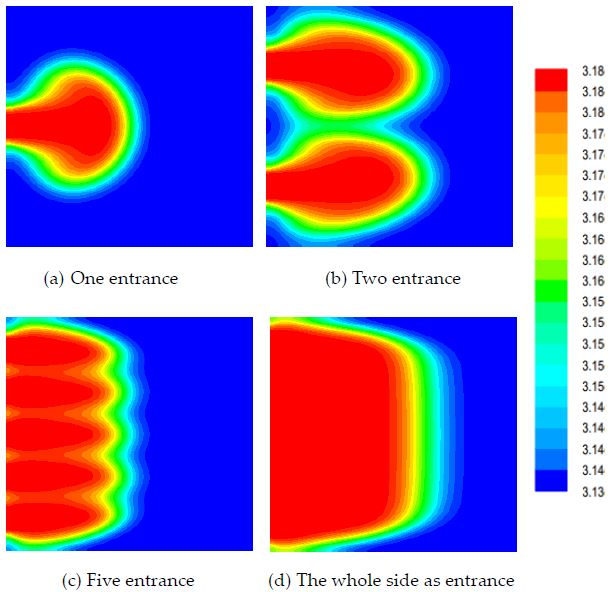
\includegraphics[width=12cm]{fig24.jpg}
\caption{The simulation results of different ways of arranging entrances} \label{fig24}
\end{figure}

From the above figure, the more the entrances are, the evener the temperature will be. Recalling on the before simulation outcome, when there is only one entrance for inflow, the temperature of corners is quietly lower than the middle area.

In conclusion, if we design more entrances, it will be easier to realize the goal to keep temperature even throughout the bathtub.

\item Model Application

Our before discussion is based on ideal assumptions. In reality, we have to make some corrections and improvement.

\begin{itemize}
\item[1)] Adding hot water continually with the mass flow of 0.16 kg/s. This way can ensure even mean temperature throughout the bathtub and waste less water.

\item[2)] The manufacturers can design an intelligent control system to monitor the temperature so that users can get more enjoyable bath experience.

\item[3)] We recommend users to add bubble additives to slow down the water being cooler and help cleanse. The additives with lower thermal conductivity are optimal.

\item[4)] The study method of our establishing model can be applied in other area relative to convection heat transfer, such as air conditioners.
\end{itemize}
\end{itemize}

\begin{thebibliography}{99}
\addcontentsline{toc}{section}{Reference}

\bibitem{1} Gi-Beum Kim. Change of the Warm Water Temperature for the Development of Smart Healthecare Bathing System. Hwahak konghak. 2006, 44(3): 270-276.
\bibitem{2} \url{https://en.wikipedia.org/wiki/Convective_heat_transfer#Newton.27s_law_of_cooling}
\bibitem{3} \url{https://en.wikipedia.org/wiki/Navier\%E2\%80\%93Stokes_equations}
\bibitem{4} \url{https://en.wikipedia.org/wiki/Computational_fluid_dynamics}
\bibitem{5} Holman J P. Heat Transfer (9th ed.), New York: McGraw-Hill, 2002. 
\bibitem{6} Liu Weiguo, Chen Zhaoping, ZhangYin. Matlab program design and application. Beijing: Higher education press, 2002. (In Chinese)

\end{thebibliography}

\newpage

\begin{letter}{Enjoy Your Bath Time!}

From simulation results of real-life situations, we find it takes a period of time for the inflow hot water to spread throughout the bathtub. During this process, the bath water continues transferring heat into air, bathtub and the person in bathtub. The difference between heat transfer capacity makes the temperature of various areas to be different. So that it is difficult to get an evenly maintained temperature throughout the bath water.

In order to enjoy a comfortable bath with even temperature of bath water and without wasting too much water, we propose the following suggestions.

\begin{itemize}
\item Adding hot water consistently
\item Using smaller bathtub if possible
\item Decreasing motions during bath
\item Using bubble bath additives
\item Arranging more faucets of inflow
\end{itemize}

\vspace{\parskip}

Sincerely yours,

Your friends

\end{letter}

\newpage

\begin{appendices}

\section{First appendix}

In addition, your report must include a letter to the Chief Financial Officer (CFO) of the Goodgrant Foundation, Mr. Alpha Chiang, that describes the optimal investment strategy, your modeling approach and major results, and a brief discussion of your proposed concept of a return-on-investment (ROI). This letter should be no more than two pages in length.

Here are simulation programmes we used in our model as follow.\\

\textbf{\textcolor[rgb]{0.98,0.00,0.00}{Input matlab source:}}
\lstinputlisting[language=Matlab]{./code/mcmthesis-matlab1.m}

\section{Second appendix}

some more text \textcolor[rgb]{0.98,0.00,0.00}{\textbf{Input C++ source:}}
\lstinputlisting[language=C++]{./code/mcmthesis-sudoku.cpp}

\end{appendices}

\newpage
\newcounter{lastpage}
\setcounter{lastpage}{\value{page}}
\thispagestyle{empty} 

\section*{Report on Use of AI}

\begin{enumerate}
\item OpenAI ChatGPT (Nov 5, 2023 version, ChatGPT-4,) 
\begin{description}
\item[Query1:] <insert the exact wording you input into the AI tool> 
\item[Output:] <insert the complete output from the AI tool>
\end{description}
\item OpenAI Ernie (Nov 5, 2023 version, Ernie 4.0) 
\begin{description}
\item[Query1:] <insert the exact wording of any subsequent input into the AI tool> 
\item[Output:] <insert the complete output from the second query>
\end{description}
\item Github CoPilot (Feb 3, 2024 version) 
\begin{description}
\item[Query1:] <insert the exact wording you input into the AI tool> 
\item[Output:] <insert the complete output from the AI tool>
\end{description}
\item Google Bard (Feb 2, 2024 version) 
\begin{description}
\item[Query1:] <insert the exact wording of your query> 
\item[Output:] <insert the complete output from the AI tool>
\end{description}
\end{enumerate}

% 重置页码
\clearpage
\setcounter{page}{\value{lastpage}}

\end{document}
%%
%% This work consists of these files mcmthesis.dtx,
%%                                   figures/ and
%%                                   code/,
%% and the derived files             mcmthesis.cls,
%%                                   mcmthesis-demo.tex,
%%                                   README,
%%                                   LICENSE,
%%                                   mcmthesis.pdf and
%%                                   mcmthesis-demo.pdf.
%%
%% End of file `mcmthesis-demo.tex'.
